\documentclass[sigconf]{acmart}
% \documentclass[letterpaper,twocolumn,10pt]{article}
%\usepackage{usenix-2020-09}
\usepackage{graphicx}
\usepackage{subfig}
%Removing the geometry package used for Tighter Format
%\usepackage{geometry}
%\usepackage{times}
\usepackage{textcomp}
\usepackage{multirow}
\usepackage{framed}
\usepackage{amsmath}
\usepackage{listings}
\usepackage{comment}
\usepackage{microtype}

\usepackage[noend]{algpseudocode}
\usepackage[nothing]{algorithm}

% \usepackage[hyphens]{url}
\PassOptionsToPackage{hyphens}{url}
\usepackage{hyperref}
%\usepackage{hyperref}
\usepackage{enumitem}
\usepackage{amssymb}

%Used only for breaking hypenated URLs
\usepackage{etoolbox}
\gappto{\UrlBreaks}{\UrlOrds}
%

\fancyhead{}
\hypersetup{breaklinks=true}

\urlstyle{same}

\copyrightyear{2023}
\acmYear{2023}
\setcopyright{acmlicensed}
\acmConference[HPDC '23]{Proceedings of the 32nd International Symposium on High-Performance Parallel and Distributed Computing}{June 16--23, 2023}{Orlando, FL, USA}
\acmBooktitle{Proceedings of the 32nd International Symposium on High-Performance Parallel and Distributed Computing (HPDC '23), June 16--23, 2023, Orlando, FL, USA}
\acmPrice{15.00}
\acmDOI{10.1145/3588195.3592995}
\acmISBN{979-8-4007-0155-9/23/06}

\newcommand{\sysname}{Il\'{u}vatar} % \xspace}

\newcommand{\alex}[1]{}
\renewcommand{\alex}[1]{{\color{red} ALEX: {#1}}}

\newcommand{\abdul}[1]{}
\renewcommand{\abdul}[1]{{\color{blue} ABDUL: {#1}}}

\newcommand{\todo}[1]{}
\renewcommand{\todo}[1]{{\color{gray} ALEX: {#1}}}

\begin{document}
\date{}

\title{\sysname: A Fast Control Plane for Serverless Computing}
%\title{\sysname: Functions as a Service made fast}

% \author{Paper Type: Open-source tools or data} % Regular 
\author{Alexander Fuerst}
\affiliation{%
 \institution{Indiana University}
 \city{Bloomington}
 \state{Indiana}
 \country{USA}
}
\email{alfuerst@iu.edu}

\author{Abdul Rehman}
\affiliation{%
 \institution{Indiana University}
 \city{Bloomington}
 \state{Indiana}
 \country{USA}
}
\email{abrehman@iu.edu}

\author{Prateek Sharma}
\affiliation{%
 \institution{Indiana University}
 \city{Bloomington}
 \state{Indiana}
 \country{USA}
}
\email{prateeks@iu.edu}

\begin{CCSXML}
  <ccs2012>
     <concept>
         <concept_id>10010520.10010521.10010537.10003100</concept_id>
         <concept_desc>Computer systems organization~Cloud computing</concept_desc>
         <concept_significance>500</concept_significance>
         </concept>
     <concept>
         <concept_id>10011007.10010940.10010971.10011120.10003100</concept_id>
         <concept_desc>Software and its engineering~Cloud computing</concept_desc>
         <concept_significance>500</concept_significance>
         </concept>
     <concept>
         <concept_id>10011007.10011006.10011072</concept_id>
         <concept_desc>Software and its engineering~Software libraries and repositories</concept_desc>
         <concept_significance>100</concept_significance>
         </concept>
     <concept>
         <concept_id>10010147.10010341.10010349.10010354</concept_id>
         <concept_desc>Computing methodologies~Discrete-event simulation</concept_desc>
         <concept_significance>300</concept_significance>
         </concept>
   </ccs2012>
\end{CCSXML}
  
\ccsdesc[500]{Computer systems organization~Cloud computing}
\ccsdesc[500]{Software and its engineering~Cloud computing}
\ccsdesc[100]{Software and its engineering~Software libraries and repositories}
\ccsdesc[300]{Computing methodologies~Discrete-event simulation}

\settopmatter{printacmref=true}

\keywords{Cloud computing; Serverless computing; Functions as a service; Open source}

\begin{abstract}
  
Functions as a Service (also called serverless computing) promises to revolutionize how applications use cloud resources. 
However, functions suffer from cold-start problems due to the overhead of initializing their code and data dependencies before they can start executing. 
Keeping functions alive and warm after they have finished execution can alleviate the cold-start overhead. 
Keep-alive policies must keep functions alive based on their resource and usage characteristics, which is challenging due to the diversity in FaaS workloads. 


Our insight is that keep-alive is analogous to caching.
Our caching-inspired Greedy-Dual keep-alive policy can be effective in reducing the cold-start overhead by more than $3\times$ compared to current approaches. 
Caching concepts such as reuse distances and hit-ratio curves can also be used for auto-scaled server resource provisioning, which can reduce the resource requirement of FaaS providers by $30\%$ for real-world dynamic workloads. 
We implement caching-based keep-alive and resource provisioning policies in our FaasCache system, which is based on OpenWhisk. 
We hope that our caching analogy opens the door to more principled and optimized keep-alive and resource provisioning techniques for future FaaS workloads and platforms. 



%%% Local Variables:
%%% mode: latex
%%% TeX-master: "paper"
%%% End:

\end{abstract}

\maketitle

\footnotetext{\sysname~is the single omniscient and omnipotent creator in Lord of the Rings.}

\section{Introduction}

Function as a Service (also called FaaS or serverless computing) is one of the fastest growing abstractions in cloud computing today with usage increasing by 2x in the past two years alone~\cite{wen2023rise}.
% Users create self-contained \textit{functions} whose lifecycle is orchestrated by the FaaS provider.  
Users are enticed by its dynamic scaling, low cost, and ease of management, as the lifecycle of self-contained \textit{functions} is orchestrated by the FaaS provider.
% Cloud providers benefit because functions use ephemeral resources unlike traditional virtual machines (VMs) and the provider has find-grained control over scheduling and placement.
Cloud providers leverage the ephemeral nature of functions into fine-grained control over scheduling, placement, and resource allocation.

% 1)
Current FaaS applications are limited by the capabilities exposed by providers, mostly consisting of short-running functions~\cite{shahrad2020serverless} using limited compute.
% Functions are given limited CPU resources and have no way efficient of coordinating with one another, precluding classic parallel computing.
Providers have not exposed GPUs or other parallel processing paradigms to their serverless platforms, a need for which is growing as users migrate new, intensive, workflows to cloud FaaS.
These applications see a \emph{minimum} 2.5x throughput improvement when accelerated, strong encouragement to enable such devices in serverless platforms.

% 2-3)
Accomplishing this transition requires the control plane to address several resource management problems.
Achieving high device utilization and low latency require device multiplexing~\cite{pemberton2022kernel, ng2023paella, fingler2022dgsf, gu2023fast}, but unmodified functions preclude such sharing of GPU resources.
% To make matters more complicated, GPU resources are managed by an esoteric device driver that isn't controllable by the OS.
Once a function is given access to the GPU, it can allocate the entire memory range or hog compute in a run-to-completion model.
% Idle periods mean allocated resources on the GPU are blocked off, other functions being unable to use them for their executions.
% Removing containers to release held resources results in heavy churn and increased latency from the repeated container initialization.
Swapping functions requires starting a new container, costing several seconds on the critical path, making the well-known \quotes{cold start} problem of FaaS an even larger latency bottleneck.
% We avoid cold starts by being the first to enable GPU keep-alive~\cite{faascache-asplos21} policies via GPU resource multiplexing.
Avoiding cold starts (i.e. a warm start) to get viable performance requires enabling GPU keep-alive~\cite{faascache-asplos21} policies via GPU resource multiplexing.

\begin{comment}
Machines used to host FaaS systems are expected to serve thousands of unique functions with low latency.
This is accomplished by running user function code inside a container (or VM), then keeping the container in memory but idle for future uses. 
A na\"ive adaption of this to the GPU problem would assign an entire GPU to each container for its lifetime.
Unfortunately an idle container then wastes GPU resources, and the limited number of GPUs per server leads to churn when we need to create a new container for another function.
% but this causes low utilization and high turnover when going to run a new function.
Virtualization for these devices exists, provisioning fixed slices of GPU resources to containers that they then have exclusive access to.
% This also results in low utilization, as nothing else can use that section when it is idle, and also limits the resources available to give to any one function that might take advantage of them.
While allowing more containers to exist concurrently, this solution does not address idleness and introduces a new limitation by reducing the maximum allocation any single function is allowed to make.
\end{comment}
  
% 4-6)
Multiplexed resources are not a performance panacea: the platform must now contend with function fairness and locality.
% The FaaS control plane must also guarantee that all functions will run in a timely and fair manner.
% GPUs must also be shared temporally 
Optimal performance is achieved by running one function repeatedly, as its data dependencies will be available on-device.
Yet a popular function can easily starve others of device time and violate fairness guarantees if not eventually blocked.
% Temporal GPU sharing between the highly heterogeneous serverless workloads must be balanced with execution \quotes{locality}.
New queuing policies tailored to the unique scenario of GPU-serverless computing must be designed to ensure fairness while maintaining high throughput.
% Warm hits, i.e. executing using an already existing container, have up to 100x lower latency compared to their cold counterparts.
% Such execution \quotes{locality} can only come 
% want warm starts.
% locality good -> 'batching'.
% but need spatial/temporal multiplexing as well.

% 7
Previous research work into enabling GPU acceleration in FaaS has focused on ML inference~\cite{pemberton2022kernel, ng2023paella, fingler2022dgsf, gu2023fast}; understandable given its popularity.
These approaches have abandoned the black-box nature of FaaS in favor of extremely fine-grained control of GPU usage and scheduling.
Supporting functions of all types is critical, as more use cases like scientific computing~\cite{kumanov2018serverless,hung2019rapid}, video encoding~\cite{ao2018sprocket, zhang2019video}, and optimization problems~\cite{aytekin2019harnessing,werner2018serverless,shankar2020serverless}, migrate to the platform.
% Our work uniquely enables all these to run natively with minimal overhead.
% Custom solutions have been proposed~\cite{}, but rely on targeted workloads or bespoke platforms, a general-purpose approach is needed.

% 7)
Given these known problems, in this work we seek to answer several research questions:
\begin{enumerate}[leftmargin=*]
  % \item Can we provide GPU acceleration to black-box, unmodified, serverless functions?
  % \item How can GPU support be integrated into high-performance FaaS control planes?
  \item Can we provide GPU acceleration to black-box, unmodified, serverless functions?
  \item Can we multiplex GPU resources between functions in a low overhead manner?
  \item How do we balance locality, fairness, and performance in the face of heterogeneous functions?
  % \item Is this possible without the cost of full virtualization?
\end{enumerate}
% \todo{Better RQs to frame novelty}

In this work, we propose and designed a series of techniques and policies that resolve all of these issues.
They enable black-box serverless functions to utilize GPUs for acceleration while concurrently sharing its resources.
We built our system on top of the \sysname~platform~\cite{fuerst2023iluvatar}, utilizing Nvidia's integration with Docker~\cite{docker-main}. %, but is generic to any accelerator or isolation system.
Importantly, they don't rely on specific hardware or software versioning support, and work on heterogeneous hardware regardless of age or capability. 

% \mhead{RQ1}
Starting from the lowest level component, we interpose an intercept shim between function code and the GPU driver.
Using this, we capture all memory allocation calls and transform them into Unified Virtual Memory (UVM)~\cite{nvidia-uvm} calls.
UVM memory allows applications to allocate beyond the device limits, letting the driver use host memory as swap space, migrating memory on demand. 
Once all allocations are converted to UVM memory, we use the shim to move memory between host and device under direction from the control plane.

% \mhead{RQ2}
Controlling memory positioning allows us to both oversubscribe device memory and keep containers warm while other functions execute on the GPU.
To enable multiple functions to run concurrently, a new queuing policy is required that better matches the new device's capabilities and workload characteristics.
We accomplish this with a modified implementation of a Mutli-Queue Fair Queue (MQFQ)~\cite{hedayati2019multi}, which prevents starvation, scales invocations across multiple GPUs, and minimizes execution overhead.
To prevent contention interference, we monitor device utilization using NVML~\cite{nvml} and track memory usage to throttle invocations.

With these controls we improve function latency by orders of magnitude over previous solutions and expand the pool of serverless applications.
In short, this work proposes the following enhancements to serverless computing:
\begin{enumerate}[leftmargin=*]
  \item We create a custom driver that intercepts function allocation calls to multiplex device memory.
  \item With no limit on device memory, we can keep idle containers resident, creating the first warm pool of GPU containers.
  \item Our memory management techniques allow us to reduce device pressure from idle functions, mitigating overcommitment overhead.
  \item We design a queuing policy that enables concurrent execution while ensuring fairness under heterogeneous workloads.
  % \item W
  % \item Benchmark suite of GPU-enabled serverless functions, including many non-machine learning applications.
\end{enumerate}

This paper is ordered as follows.
Section~\ref{sec:bg} covers background of serverless work and GPU virtualization.
Our motivation behind work is explained in detail in Section~\ref{sec:motiv}.
Section~\ref{sec:design} details our design of queuing, memory control, and resource management.
We examine the implementation of these pieces in Section~\ref{sec:impl}.
Lastly, Section~\ref{sec:eval} shows the effectiveness of our systems with a thorough experiment suite.

% \vspace*{-8pt}
\section{Background \& Motivation}
\label{sec:bg}
%\subsection{Functions as a Service}
%\label{sec:bg:faas}

Functions as a Service (FaaS) allows users to register small snippets of function code that get executed in response to some event or trigger (such as an HTTP request, message queue event, etc.)
~\cite{serverless-cacm-21, aws-lambda, google-functions,azure-functions}. 
These functions must be stateless: a new execution environment may be created for every invocation (and can be destroyed after the function returns). 
The function code also contains all the necessary code and data dependencies (such as imported libraries and packages), and thus functions may spend significant time being \emph{initialized} before the event-handling code can execute. 
Functions are executed inside virtual execution environments such as hardware virtual machines, OS containers like Docker, or even language-based runtimes such as javascript WASM~\cite{shillaker2020faasm}.
Function initialization, i.e., creating the execution environment and resolving code/data dependencies, can take 100s of milliseconds, and this ``cold-start'' can significantly increase the latency of small functions~\cite{du2020catalyzer, faascache-asplos21}.
Initialized function sandboxes can be retained in memory, and this \emph{keep-alive} provides faster ``warm-starts''~\cite{faascache-asplos21}. 
%
Since functions are arbitrary user-code, they are extremely heterogeneous in their execution characteristics and resource requirements. 
% For instance, the FaaS workload traces provided by Azure shows that the workload is buextremely bursty and heavy-tailed across many dimensions: a small fraction of functions are responsible for a majority of invocations, and some large functions contribute to a majority of the resource consumption.
For instance, the Azure FaaS trace~\cite{shahrad_serverless_2020} shows that the 50th and 95th percentile of execution time can range from 1 second to 1 minute; and the inter-arrival-time from 1 second to 15 minutes respectively.

% \vspace*{-8pt}
\subsection{FaaS Control Planes}
\label{sec:bg:cplane}

All aspects of function execution are orchestrated by a FaaS \emph{control plane}, which are implemented by frameworks like OpenWhisk~\cite{openwhisk}.
For using a FaaS service, the user interacts with the control plane for registering and invoking functions, tracking their status, etc.
The control plane manages the resources of a cluster of servers, and schedules functions on to them based on its load-balancing policies.

%FaaS is a relatively new workload paradigm, and control planes are still evolving and maturing.
%OpenWhisk is a popular framework which has been used as a platform for investigating and optimizing many facets of FaaS execution.

In OpenWhisk, user requests for invoking a function go through a reverse proxy (NGINX) to the central \emph{controller}, which implements, among other things, load-balancing (a variant of consistent hashing with bounded loads by default).
The controller puts the function invocation request into a shared Apache Kafka~\cite{kafka} queue.
Inside the worker, the invoker service pulls function invocations from the Kafka queue based on that worker's own resource availability.
Docker containers running a Go-based control plane agent are used to isolate functions, and each worker maintains a container pool of initialized/warm containers.
% A worker ultimately runs the function, and the control plane extends across the worker as well. 
%OpenWhisk strives to provide exactly-once semantics (although this hasn't been tested or verified) by logging function results in CouchDB. Kafka and CouchDB in the critical path. 
OpenWhisk logs function results in a CouchDB instance.
Importantly, both Kafka and CouchDB are on the critical path, and add 100s of ms to invocation latency.
%
OpenWhisk is highly modular and distributed, with many networked services.
All of these, combined with the JVM GC (it is implemented in Scala), results in large and unpredictable latency spikes~\cite{faaslb-hpdc22, hotcarbon22-faas}, with slowdowns of more than $10,000\times$ reported~\cite{zuk_call_2022}. 
%For instance, Stretch factors shown in \cite{zuk} of 10,000, indicating that the overhead is 10,000 more than the actual processing latency, and with response times of 100s of seconds. 

\begin{comment}
Shared kafka queue for scheduling and assignment of invocations.
Contended.
Ours simpler design: locality enforced through multiple independent loosely coupled components: CH-BL load balancer, and queuing at the invoker for tolerating bursts. 

The burst mitigation is done again using many techniques.
Increase queue size, overcommit resources and increase concurrency, forward, and finally elastic scaling.

OS level preemption is useful, since function invocation is not confined to a single process but many components such as containerization layer. The resource usage is also not uniform, but bursty and low average.

Stretch factors shown in \cite{zuk} of 10,000, indicating that the overhead is 10,000 more than the actual processing latency, and with response times of 100s of seconds. 

\noindent \textbf{Control planes}  (such as OpenWhisk~\cite{openwhisk})  handle all aspects of function execution. 
This control plane manages a cluster of servers to run functions on, and implements function scheduling, load-balancing, resource monitoring, function status tracking, storing function results, logging, etc. 
It is also responsible for performance optimizations for functions such as keep-alive~\cite{faascache-asplos21} to mitigate function cold-start overheads due to the sandboxing and function initialization overheads. 
%\emph{Paint a picture of what all it does.}
The control plane itself is highly distributed with many components such as API gateways, distributed message queues (such as Kafka), and databases. % (like CouchDB).
Even on a single server, a function's execution is orchestrated through many components, as shown in Figure~\ref{fig:faasmeter-iluvatar}. 
\end{comment}

% \vspace*{-8pt}
\subsection{Why a new FaaS control plane?}
\label{sec:bg:ynew}

% Why did we embark on this mission in the first place?

We believe that the FaaS control plane is an important component of the modern cloud ecosystem, and presents many optimization opportunities and interesting research questions in system design. 

\begin{figure}
  \centering  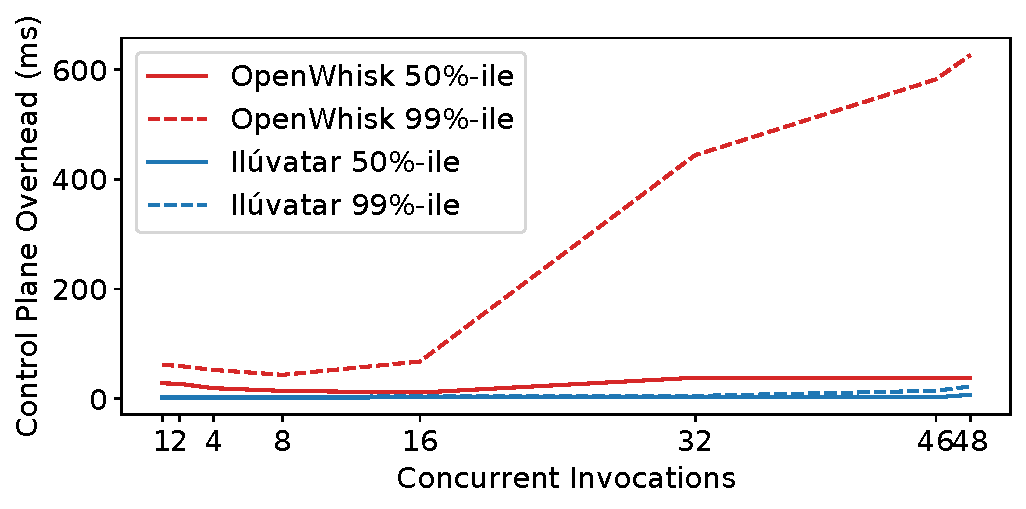
\includegraphics[width=0.4\textwidth]{iluvatar/graphs/scaling/pyaes/overhead-scaling.pdf}
  % \vspace*{-6pt}
  \caption{The latency overhead of the control plane, as the number of concurrent invocations increases. OpenWhisk overhead is significant and has high variance, resulting in high tail latency. \sysname~ reduces this overhead by 100x. }
  \label{fig:ow-scaling}
    % \vspace*{-6pt}
\end{figure}


\noindent \textbf{Performance.}
%
Because of its central role in coordinating all aspects of function execution, the control plane plays a major role in determining function performance. 
Managing the function execution lifecycle for hundreds of concurrent invocations imposes a \emph{control plane overhead}, and increases the end-to-end latency.
This control plane overhead can be significant, and affects \emph{all} function invocations, including and especially the ``warm starts''. 
%Time spent in the control plane is simply measured by subtracting the execution time of the function code from the overall end-to-end latency.
This overhead (end-to-end latency minus the function code execution time) for the PyAES function from FunctionBench~\cite{kim2019functionbench} is shown in Figure~\ref{fig:ow-scaling}. 

The figure shows the 50 and 99 percentile overheads as the number of concurrent invocations are increased.
In each case, we are invoking the function repeatedly in a closed-loop, and concurrent invocations are achieved by using multiple client threads.
All invocations are warm starts.
The experiment is run on a 48 core server (more details in Section~\ref{sec:eval}), and the figure thus shows the performance at low and medium load conditions. 

From Figure~\ref{fig:ow-scaling}, we can see that the OpenWhisk latency overhead is more than 10ms,  which is already a significant increase in latency for small functions which dominate real-world FaaS workloads.
Worryingly, the 99 percentile overhead is much higher, and rises to as much as 600ms.
We also see strange inversions in the scaling behavior: the overhead reduces for certain load-levels, and then increases again.
This high overhead, high variance, and uncertain scaling behavior, results in many challenges for FaaS \emph{providers}. 
Due to these issues, low-latency functions see severe performance degradation, and resource provisioning and capacity planning becomes harder due to the high variance and performance unpredictability. 
%

Some of these latency overheads are an artifact of the architecture. 
The shared Kafka function queue can be a major bottleneck; and there are no explicit backpressure or load regulation mechanisms, which is compounded by the CPU overcommitment. 
%
For the sake of comparison, the figure also shows the latency overhead of \sysname~ in the same environment. 
We are able to achieve a per-invocation mean overhead of less than 2ms for almost all the load conditions.
Importantly, the tail overhead is also small: less than 3ms for less than 32 concurrent invocations, rising to 10ms when the system is saturated.


To emphasize, for a median function in the Azure workload which runs for 500 ms, OpenWhisk can increase its latency by 100\%.  
Thus, the control plane plays a crucial role in function performance.
We note that these are the best-case warm-start latencies, when the function's containers is fully initialized and in memory. 
Since function cold-starts impose such a major performance penalty (increasing latency by more than $10\times$), mitigating them has been a major research focus. 
However, because of temporal and spatial locality of access, caching and prefetching techniques can be extremely effective, and the cold-start rate is often less than $1\% $ of all invocations~\cite{faascache-asplos21}. 
The majority of invocations are thus ``warm'', where the performance is dominated by control plane overheads.
%\emph{We thus need a low-latency, low-jitter control plane.}

\noindent \textbf{System Design.}
%
As evidenced by the OpenWhisk architecture presented earlier, FaaS control planes are large, complex distributed systems.
Due to the continually evolving needs of FaaS applications and emergence of new sandboxing techniques (such as lightweight VMs like Firecracker~\cite{firecracker-nsdi20}), they are sandwiched between the scale and heterogeneity of FaaS workloads on one hand, and the deep stack of OS and virtualization components on the other. 

For instance, systems for running web services or microservices do not have to deal with large and highly variable sandbox management overheads, nor with highly heterogeneous request sizes.
For reducing tail latency, these systems can often rely on the OS CPU scheduler for processor sharing, can do CPU allocation at very fine granularity~\cite{kaffes2019shinjuku}, use queuing theory techniques~\cite{prekas2017zygos}, etc. 
At the other extreme, for longer running containers and VMs, their control planes, like OpenStack or Kubernetes face a much lower rate of VM arrivals and departures. and can do careful and ``hard'' resource allocation using bin-packing~\cite{cortez2017resource}.


Functions are highly heterogeneous, and can be seen as both latency-sensitive web requests \emph{and} large containers requiring significant system resources for several seconds. 
FaaS control planes thus have to do \emph{both} low-latency allocation \emph{and} pack CPU and memory resources on their servers carefully to maintain high system utilization.
%
%We posit that these competing needs present new challenges in large-scale distributed resource allocation.
Thus FaaS control planes are one of the more perfect microcosms of challenges in resource management and control in large scale distributed computing. 

A clean-slate control plane design helps us investigate the fundamental performance tradeoffs and challenges in this fast-evolving ecosystem.
Our new implementation also helps to identify the current performance bottlenecks and new avenues of OS optimizations. 


\noindent \textbf{Platform for Experimental Systems Research.}
%
Performance-focused FaaS research is already challenging due to the extreme scale and heterogeneity of the workloads.
These challenges are compounded by existing control planes like OpenWhisk that are unfortunately highly unpredictable.
The control plane jitter and the extreme bimodal cold vs. warm latencies makes it difficult to do reliable and reproducible research~\cite{mytkowicz2009producing}, and subtle environmental and configuration effects can mask the true effects of new research optimizations.
However, it continues to be a key component in developing and evaluating FaaS research~\cite{akkus_sand_2018, shahrad_serverless_2020, faascache-asplos21, faaslb-hpdc22, zhou2022aquatope, ensure-faas-acsos20, alzayat_groundhog_2022}. 
%OpenWhisk is a popular framework which has been used as a platform for investigating and optimizing many facets of FaaS execution.
With OpenWhisk, function performance can be severely affected by a myriad of configuration options, such as insufficient memory for CouchDB, networking configuration, Docker configuration, etc. 

Given the importance of the control plane, we want \emph{predictable} performance to a large degree. 
In our experience, research in FaaS is often hindered by the large overheads and complexity of existing control planes. 
Thus, \sysname~ is designed from the ground-up to be lightweight and provide predictable performance under different conditions. 
Our system implementation can potentially accelerate the development of new optimizations, clarify  our understanding of performance characteristics of this relatively new stack, and provide a platform for robust experiments. 
% Establishing a shared open platform enables easy comparison between research work
With a robust platform, the community can share knowledge and advances, while being able to compare against a well-known and trusted baseline.

\begin{comment}
\textbf{Why write from scratch instead of improving existing ones?}

A clean-slate design also gives us the opportunity for understanding the design tradeoffs that could be helpful for general FaaS research and 

Lightweight/minimal ones like faasd exist. But again, written in go, not performance focused, and implementing all the desired research features would make it a different.

We also wanted this to be a design exercise in exploring the tradeoff between being lightweight and high performance vs. being extensible and ``full-featured''.
\end{comment}


%%% Local Variables:
%%% mode: latex
%%% TeX-master: "paper"
%%% End:

% \vspace*{-8pt}
\section{\sysname~ Design}
\label{sec:design}

% Design goals:
%   A research platform
%     Easy to use, adjust source code, modification points
%     Full system stack: controller (load balancer), worker(s), load generation, containers, workloads, simulation
%     Configurable, lots of knobs to adjust things easily
%     Tracking of metrics/resources/system events
%   low-variance! and low(ish)-overhead platform
%   No frivilous features, not too complicated

\sysname's design is guided by our experience of OpenWhisk performance, and by our goals of providing predictable performance, modularity, and a platform for reliable FaaS research.

% \vspace*{-8pt}
\subsection{Architecture and Overview}
\label{sec:design:arch}

The \sysname~ control plane is spread out across a load balancer and the individual workers, and sits above the containerization layers. 
We intend for \sysname~ to be the narrow waist~\cite{popa_http_2010} in the FaaS ecosystem: with optimizations for DAG scheduling~\cite{zhou_qos-aware_2022}, state handling~\cite{sreekanti2020cloudburst}, and horizontal scaling~\cite{faaslb-hpdc22} implemented above it, and sandboxing and containerization below it.  
This architecture was motivated by the key question: \emph{Can fast FaaS control planes be implemented with strict layering and separation of concerns?}


We have found that most of the control plane overhead is in the workers, and hence optimizing the worker performance is our major focus.
%
Our architecture is \textbf{worker-centric}, and places more performance and load-management responsibility on the individual workers, instead of a more ``top-down'' centralized approach favored by prior work such as Atoll~\cite{singhvi2021atoll} and others~\cite{kaffes_centralized_2019, kaffes_hermod_2022}.
Top-down resource management requires a consistent global view of the cluster, and is complementary to our work. 
Predictive techniques for load-balancing, prefetching, scheduling, function-sizing can all be effective, but we want to explore the performance characteristics and limits of \emph{reactive} control planes that work with unmodified container runtimes. 

\begin{figure}
  \centering 
  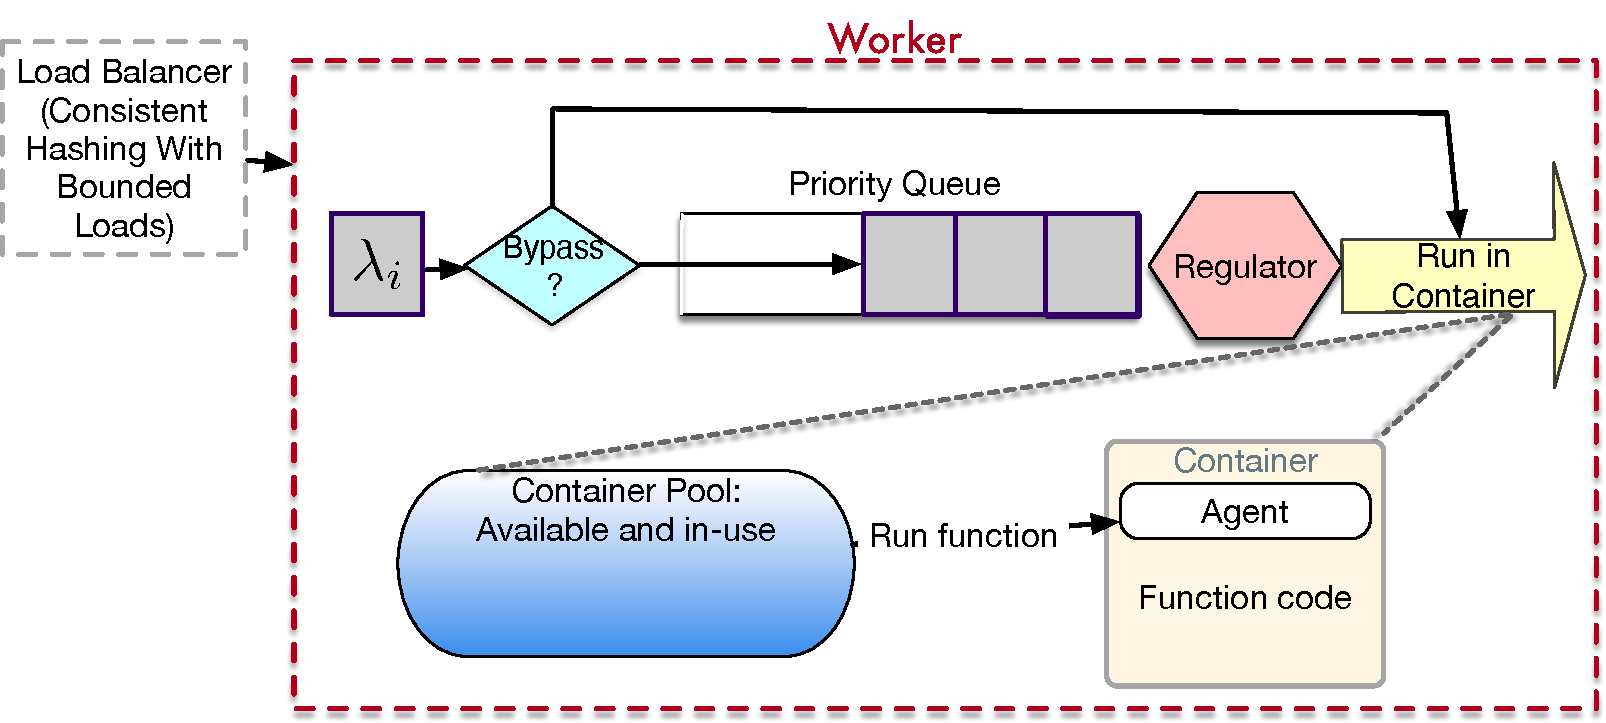
\includegraphics[width=0.6\textwidth]{iluvatar/figs/il76-q.pdf}
    % \vspace*{-6pt}
  \caption{\sysname~ has a worker-centric architecture. A per-worker queue helps schedule functions, and regulate load and overcommitment. }
  \label{fig:arch}
  % \vspace*{-6pt}
\end{figure}

\sysname's main components are shown in Figure~\ref{fig:arch}.
Clients/users invoke functions using an HTTP or RPC API, with the main operations being \texttt{register, invoke, async\_invoke, and prewarm}.
Workers also provide load and status information to the load-balancer. 
We use stateless load-balancing, by using variants of consistent hashing with bounded loads (CH-BL), which have been proposed for FaaS recently~\cite{faaslb-hpdc22}. 
This is a locality-aware scheme, which runs functions on the same servers to maximize warm starts, and forwards them to other servers only when the server's load exceeds some pre-specified load-bound.


Continuing on the worker-centric theme, the worker API is a subset and almost completely identical to the overall API, and functions can be launched directly on a worker for single-worker setups and benchmarking, without going through a load-balancer and adding unnecessary latency.
The workers implement various latency-hiding and burst-mitigation techniques. 
All functions are launched inside containers, and dealing with the container layer is a major part of the worker. 
Each worker maintains a container pool of initialized containers for facilitating warm starts, and has an invocation queue for handling dynamic loads.
Function characteristics such as their cold and warm execution times are captured in various data-structures and are made available using APIs for developing data-driven resource management policies.

An important contribution and component of \sysname~ is its principled support for function overcommitment based on its queuing architecture.
In many environments, like public FaaS providers, function resources cannot be overcommitted. 
However, the actual function resource usage is often significantly less compared to their requested ``size''.
This difference is the motivation behind recent ``right sizing'' work~\cite{akhtar_cose_2020, guo_decomposing_2022, tian_owl_2022, eismann2021sizeless, kotni2021faastlane}, and can significantly improve system utilization.
Through its queue-based architecture (described in Section~\ref{sec:q}), \sysname~ supports a wide range of overcommitment scenarios, including no overcommitment, which is absent from OpenWhisk.
By default, OpenWhisk does not overcommit memory, but can  overcommit CPUs, which introduces performance interference and potential SLA violations for functions. 



%%%%%%%%%%%%%%%%%%%%%%%%%%%%%%%%%%%%%%%%


% \subsection{Function handling in the workers}
% \vspace*{-8pt}
\subsection{Function Lifecycle}
\label{sec:design:lifecycle}

%Function lifecycle is controlled by three main \sysname~ worker API calls.
New functions need to be first \emph{registered}, which entails downloading and preparing its container disk image.
The container images are fetched from DockerHub or some other image repository.
Container images are composed of multiple copy-on-write layers, and we prepare the images by selecting the relevant layers for the operating system and CPU architecture.
The images consist of the user-provided function code and our agent, which is a simple Python HTTP server that runs in each container. 
%How functions are registered and prepared to run by the platform isn't immediately interesting research-wise, so we choose to do these out-of-band.
%
Registered functions can then be directly \emph{invoked}, which triggers launching of the function's container.
The first invocation is usually a cold start, which entails launching the container image from disk, or from a previous snapshot~\cite{ustiugov2021benchmarking, ao2022faasnap} if available. 
Each function container starts the agent which listens for and controls the actual function code execution. 
The agent has two simple commands, a \texttt{GET /} endpoint for simple status checking, and a \texttt{POST /invoke} to run an invocation with some arguments.
When the container is ready, the worker sends an HTTP request to the agent to start the function code execution. 
We detect the container's readiness using an inotify callback, which is a faster and more generic mechanism for notification compared to Docker's built-in API. 
%
Finally, when the function finishes execution, the HTTP call to the container's agent returns, and the container is marked as  `available' in the container pool, to be potentially used for future invocations of the same function.

In the spirit of a fast ``baseline'' control plane and for isolation, \sysname~ does not share containers across functions.
This is in contrast to SAND's application sandboxing~\cite{akkus_sand_2018}, SOCK's Zygote containers~\cite{oakes_sock_2018}, Nightcore~\cite{jia2021nightcore}, and even OpenFaaS~\cite{openfaas}.
%For example, recently proposed optimizations such as SAND's application sandboxing~\cite{akkus_sand_2018}, or SOCK's Zygote containers~\cite{oakes_sock_2018} share containers for concurrently running functions. 
% allow for functions to share a language runtime inside a container, or the same function to reuse 
% SAND's application sandboxing~\cite{akkus_sand_2018}, or SOCK's Zygote containers~\cite{oakes_sock_2018}. 
%We don't allow concurrent invocations of the same function to run in the same container like OpenFaaS~\cite{openfaas} or nightcore~\cite{jia2021nightcore}.
Our isolation model is similar to the public cloud providers. 

Additionally, \sysname~ introduces a standard \texttt{prewarm}  API call, which starts the function's container and the agent inside of it, and adds it to the container pool.
This reduces most of the cold start overhead associated with the container.
Prewarming can both avoid a ``thundering herd'' of cold starts on worker startup, and be an optimization in which the control plane anticipates invocations and prepares containers for them. 
This allows for a systematic mechanism to implement various recently proposed predictive prewarm policies~\cite{roy2022icebreaker, shahrad_serverless_2020, silva_prebaking_2020}. 

%When a container is created, our agent is started up inside it.




\begin{figure}
\centering 
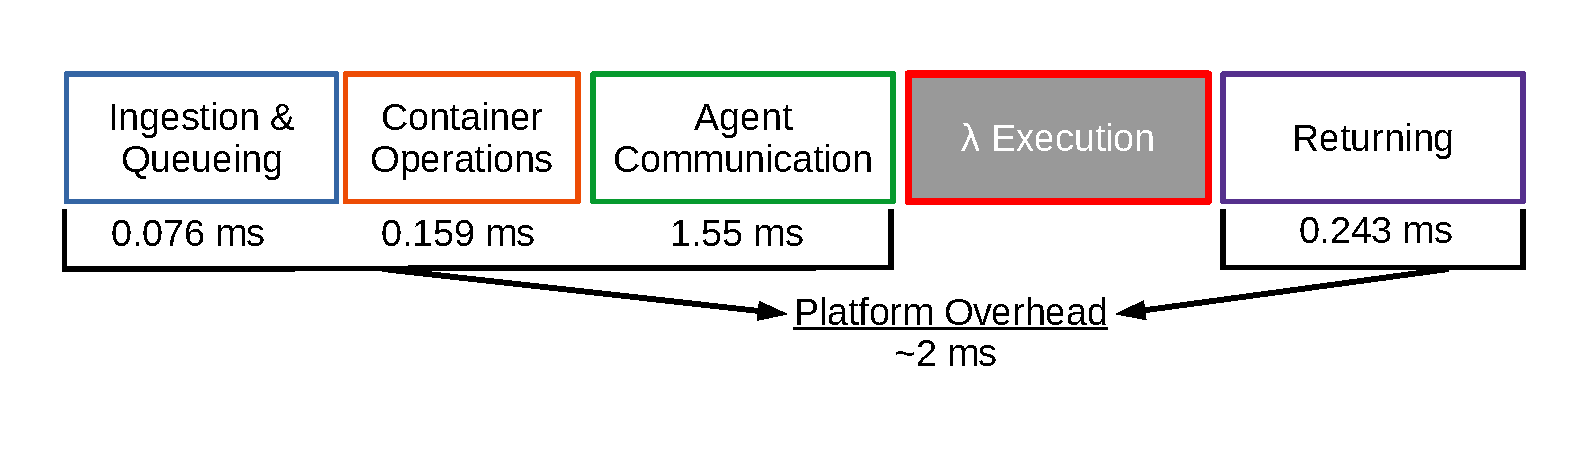
\includegraphics[width=0.6\textwidth]{iluvatar/figs/OverheadTimeline.pdf}
% \vspace*{-12pt}
\caption{The main components of the \sysname~ overheads.}
\label{fig:timeline-flow}
  % \vspace*{\myfigspace}
  % \vspace*{-12pt}
\end{figure}


\noindent \textbf{Function Latency Breakdown.}
Throughout \sysname~ and this paper, we are interested in three main performance metrics. 
The first is the end-to-end latency of function execution, also called the \emph{flow time}, shown in Figure~\ref{fig:timeline-flow}.
This in turn has two main components: the control plane overhead is the latency of \sysname~ operations, which are mainly before the start of function execution.
The second component is the function execution time, which is determined by the function code, and the load on the system.
The function execution time is our baseline, and we compute the \emph{normalized} end-to-end latency by dividing the full latency by the execution time (also called the \emph{stretch}). 

A more detailed latency breakdown is shown in Table~\ref{tab:overheads}.
The majority of overhead comes from the communication with the agent which is over HTTP. 
This is a deliberate choice, since we wanted to be compatible with existing OpenWhisk function images.
This can be reduced by using faster IPC mechanisms like in Nightcore~\cite{jia2021nightcore}. 
However, these faster communication approaches would reduce compatibility, especially with functions deployed inside VMs.

For OpenWhisk, a similar latency breakdown shows that a large amount of time is spent reading/writing to CouchDB (up to half a second), and the rest of the slowdown occurs in the Invoker (OpenWhisk's worker) and is primarily due to its design and implementation. 
Interestingly, the load-balancer/controller for OpenWhisk adds less than 3ms of latency even under heavy load, indicating that the worker-level performance is relatively more important. 
This further motivates our worker-centric design and evaluation focus. 


\begin{table}
  \begin{tabular}{|c|c|r|}
    \hline
    Group & Function Name & Time (ms) \\
    \hline
    Ingestion \& Queuing & \begin{tabular}{@{}c@{}}invoke \\ sync\_invoke \\ enqueue\_invocation \\ add\_item\_to\_q \end{tabular} & \begin{tabular}{@{}c@{}}0.026 \\ 0.013 \\ 0.017 \\ 0.02 \end{tabular} \\
    \hline
    Container Operations & \begin{tabular}{@{}c@{}}spawn\_worker \\ dequeue \\ acquire\_container \\ try\_lock\_container \\ \end{tabular} & \begin{tabular}{@{}c@{}}0.029 \\ 0.02 \\ 0.096 \\ 0.014 \\ \end{tabular} \\
    \hline
    Agent Communication & \begin{tabular}{@{}c@{}}prepare\_invoke \\ call\_container \\ download\_result \\ \end{tabular} & \begin{tabular}{@{}c@{}}0.154 \\ 1.364 \\ 0.032 \\ \end{tabular} \\
    \hline
    Returning & \begin{tabular}{@{}c@{}}return\_container \\ return\_results \\ \end{tabular} & \begin{tabular}{@{}c@{}}0.017 \\ 0.266 \\ \end{tabular} \\
    \hline
  \end{tabular}
  \caption{Latency of different \sysname~ worker components for a single warm invocation.}
    \label{tab:overheads}
\end{table}

%As we can see, the overheads are minimal. Some queuing, some agent communication, which totals to about 3ms. 
% \vspace*{-8pt}
\subsection{Worker Performance Optimizations}
\label{sec:design:worker}

To achieve this low latency function execution for heterogeneous and bursty workloads, \sysname~ uses two key underlying design  principles: resource caching, and asynchronous handling of function life-cycle events.

\subsubsection{Resource Caching}

%\noindent \textbf{Resource Caching.}
The cornerstone design goal of \sysname~ is to reduce jitter, which we accomplish by removing expensive operations from the function's critical path. 
Instead, we cache and reuse as many function resources as possible, which minimizes the ``hot path'' function invocation latency significantly.
This principle is applied in various worker components, which we describe below.

\noindent \textbf{Container Keep-alive.}
The primary and exemplary application of resource caching is in the container keep-alive cache that \sysname~ workers maintain.
The containers become ``warm'' when their function has finished execution, and become ``available'' for the next invocation of the same function. 
We maintain a pool of all in-use and available containers for each registered function.
This container cache implements classic eviction policies such as Least Recently Used (LRU), and size-aware policies like Greedy-Dual-Size-Frequency, as proposed in FaasCache~\cite{faascache-asplos21}. 

\noindent \textbf{Network Namespace Caching.}
For isolation, each container is provided with a virtual network interface and a network namespace.
Through performance profiling, we've found that creating this network namespace can add significant latency to container cold starts---as much as 100ms.
This is due to contention on a single global lock shared across all network namespaces~\cite{oakes_sock_2018}. 
To minimze this overhead, we maintain a pool of pre-created network namespaces that are assigned during container creation. 
The isolation is still maintained, since concurrently running containers do not share the namespace. 
%Avoiding this expensive operation on the critical path.

\noindent \textbf{HTTP Clients.}
The worker threads communicate with the in-container agent for launching the function code.
Instead of creating a new HTTP client for every invocation, we cache a client per container and use connection pooling. 
This affects all invocations (even warm starts), and reduces the control-plane overhead latency by up to $3ms$. 

\subsubsection{Async function life-cycle handling}

The second key design principle is to handle various aspects of the function's lifecycle asynchronously off the critical path.
\sysname~ achieves this through background worker threads for certain tasks, and through its Rust implementation which heavily uses asynchronous functions, futures, and callbacks wherever possible. 

\noindent \textbf{Keep-alive eviction.}
One such aspect is maintaining the function keep-alive cache, and ensuring that new functions have enough free memory to launch without waiting on existing containers to be evicted first.
Traditionally, eviction decisions would be made in an online fashion, but picking victims and waiting for their removal creates high variance in function execution times. 
\sysname~ performs container eviction from the keep-alive pool  periodically in the background, off the critical path. 
This is similar to the Linux kernel page-cache implementation. 
We maintain a minimum free-memory buffer for dealing with invocation bursts, and periodically sort the containers list for eviction based on caching policies from~\cite{faascache-asplos21}. 

\noindent \textbf{Function Queuing.}
An important component of \sysname's architecture is a per-worker function queue.
New invocations are first put into the queue, and are dispatched to the container backend by a queue monitoring thread. 
%only when sufficient resources are available.
This allows us to tolerate bursts of invocations, and regulate the server load. 
Details of our queuing policies are presented in Section~\ref{sec:q}.

%%%%%%%%%%%%%%%%%%%%%%%%%%%%%%
% \vspace*{-8pt}
\subsection{Container Handling}
\label{sec:design:ctr}

\sysname~ uses standard Linux containers for isolating and sandboxing function execution---a ``vanilla'' and conventional approach.  
Several exciting new isolation mechanisms for cloud functions
have been proposed: such as lightweight VMs~\cite{firecracker-nsdi20}, unikernels, WASM~\cite{shillaker2020faasm} and other language runtimes~\cite{graalvm}, etc. 
Importantly, the sandboxing affects the \emph{cold start} overheads, which account for a tiny fraction of all invocations (usually less than 1\%).
Our control plane design and performance optimizations are independent of the sandboxing mechanism, and we address the orthogonal problem of optimizing the \emph{warm starts}. 

The basic container operations we use are: i) Create a container/sandbox with specified resource limits and disk image/snapshot, ii) launch a task inside it for the agent, and iii) destroy the container.
Each container is launched with the CPU and memory resource limits. CPU limits are enforced with cgroup quotas. 
This limited API allows \sysname~ to support \emph{multiple} container backends.


By default, we use containerd~\cite{containerd}, which is popular container library, also used by Docker. 
The very rich containerization ecosystem presents a large number of options, and examining their tradeoffs was a major part of \sysname's design process.
Importantly, the choice of containerization library impacts the cold start times, and some library operations can take considerable time (100s of ms). 
High-level container frameworks like Docker are feature-rich and easy to use, but are typically used for long-running containers and are not optimized for latency.
Docker uses containerd under the hood, and it provides  more fine-grained control and slightly better latency.
Functions require a minimal containerization, and a lot of feature-complexity in these large containerization libraries can add to latency.
For instance, the crun~\cite{crun} library which is written in C takes about 150ms to launch a container, whereas containerd (written in Go) needs 300ms, and Docker needs 400ms. 

Using containerd allows us to use the OCI container specification~\cite{oci}, and makes it easier to support other container runtimes.
For instance, we also support the Docker container backend, which required only a minimal programming effort.
Containerd operates as a separate service, and we use it's RPC-based API, which contributes to some latency as well.
We contemplated writing our own optimized container runtime in Rust to avoid the overheads due to inter process communication, extra process forks and system calls, and implement other cgroups and namespace optimizations. 
However, we ended up going with containerd to keep our control plane small and reusable across container runtimes.
We also wanted to investigate and tackle the challenge of getting predictable performance out of higher level containerization services that are not part of the same address space. 


\noindent \textbf{Simulation Backend.}
In addition to containerd and Docker containers, we also support a ``null'' container backend which is useful for simulations and evaluating control plane scalability.
%
Because of the scale and variety of FaaS workloads, using discrete event simulators for developing and evaluating resource management policies is often necessary.
%
For instance, the recent work on FaaS load balancing~\cite{faaslb-hpdc22} uses such a simulator for evaluating their policies at scale for different subsets of the Azure workload trace.
Usually, the simulation is used to augment and complement the ``real'' empirical evaluation of the same policies which are implemented in FaaS frameworks like OpenWhisk. 

However, a major methodological and practical issue is that the policy implementations, workload generation, and analysis, all need to be duplicated across the simulator and the real system.
This can lead to subtle and large divergences between the simulation and real environment. 
Moreover, the simulator cannot capture all the real-world dynamics and jitter, and can suffer from poor fidelity.

In order to aid researchers, \sysname~ takes a different approach to simulations, and provides \emph{in-situ} simulations. 
Our ``null'' container backend does not run any actual function code, but instead sleeps for the function's anticipated execution time.
The rest of the control plane operates exactly as with real containers, and we still handle all other aspects of the function's lifecycle.
%
This allows us to simulate large systems and workloads. 
For evaluating any particular policy, researchers can use the simulator null-backend to evaluate control-plane overheads, warm-starts, etc., without requiring a large cluster.
Each \sysname~ worker can ``simulate'' 100s of cores, since the CPU resources are only being consumed by the control plane, and not for running actual functions.
Alternatively, a large cluster can be simulated with multiple simulated workers. 

With this approach, \emph{there is minimal difference} between the simulation and the real system. 
Thus an experiment can be run in-situ or in-silico, following identical code paths.
The main distinction is that API calls to containerd are replaced with internal dummy function calls, and function invocations are converted to sleep statements.  
All control plane operations, control-flow, logging, resource limits enforcement, etc., are exactly the same as with the ``real'' \sysname.
This also helps with mocking and testing new policies. 

%%%%%%%%%%%%%%%%%%%%%%%%%


%%% Local Variables:
%%% mode: latex
%%% TeX-master: "paper"
%%% End:

% \vspace*{-8pt}
\section{Function Invocation Queuing}
\label{sec:q}

As a way to regulate and control function execution and worker load, \sysname~ incorporates a per-worker invocation queue architecture. 
Function invocations go through this queuing system before reaching the container manager, which either locates the warm container and runs the function or creates a new container.
Each worker manages its own queue, differentiating our design from OpenWhisk's shared Kafka queue. 

\noindent \textbf{Motivation.}
%
This queuing architecture is motivated by three main factors: i) the bursty nature of the workload , and ii) Reducing cold starts due to concurrent invocations, and iii) to give workers additional mechanisms for controlling their load, implementing prioritization, etc. 
Note that once the function passes through the queue, it is effectively ``scheduled'' for execution by the OS CPU scheduler.
The CPU scheduler of course has its own throttling and controling mechanisms, such as cgroups and the various scheduler tuning knobs.
The invocation queue thus acts as a kind of a regulator or a filter before the CPU scheduler, and ideally, ``feeds'' it the right functions at the right rates for maximizing throughput and minimizing latency.
%

Because function workloads are so bursty and heterogeneous, running each function immediately can significantly increase the worker load and result in severe resource contention and increase  function tail latencies.
%
The queue also helps as an explicit back-pressure mechanism for load-balancing, admission control, and elastic scaling.
The queue length is  used for accurately determining the true load on the worker, which is a vital input to consistent hashing with bounded loads~\cite{faaslb-hpdc22}.
This reduces the staleness and noise of using system load average as the load indicator, and makes load balancing more robust.


Queuing invocations also allows us to reduce cold starts.
While repeated function invocations are good and increase warm starts, 
\emph{concurrent} invocations of the same function results in cold starts for all the concurrent invocations, since each invocation needs to be run in its own container.
This is also the ``spawn start''~\cite{ristov_colder_warmer}, which causes severe latency increase of 10s of  seconds in public FaaS. 
If there are $n$ concurrent invocations that arrive at the same time, then the $n$ concurrent cold starts can significantly increase the system load and affect latency of other functions.
Instead, by queuing and throttling the functions, we can wait for the invocation to finish, and then use the warm container for the next function in this ``herd'', and so on and so forth. % Lol zizek 
%Having a queue allows us to regulate the invocations by this and other means. (?) 

% \vspace*{-8pt}
\subsection{Queue Architecture}
\label{sec:q:arch}

\sysname's queue architecture is shown in Figure~\ref{fig:arch}.
We have three main components.
%
From right to left, first, we have a concurrency regulator (or just regulator), which enforces the \textbf{concurrency limit}: the  upper-bound on the number of concurrently running functions. 
%
This lets functions execute ``on cpu'' without timesharing, and effectively determines the overcommitment ratio.
Higher concurrency limits (more than the number of CPUs) means  more CPU overcommitment.
Note that even with overcommitment, the cgroup quotas still provide proportional allocation (thus a 2 CPU container will still get twice the CPU cycles compared to a 1 CPU container). 
%
In addition to concurrency, other factors can also be used to regulate the queue discharge rate. 
The regulator can be used to run functions of only when sufficient resources (such as CPU bandwidth, warm containers, or even accelerators like GPUs) are available. 


%Note that technically the queue service backend is a processor sharing system, so can tolerate immediate execution albiet under heavy load.
%The concurrent cold start mitigation is one important component of the regulator policy.
%Its inputs are the number of currently running functions, the state of the container map to see which functions are executing, and the system resource utilization (load average, cpu\%, etc).
%This allows custom policies: we may want to limit the load average to under some limit, or the number of functions ``in flight'', etc.
\sysname~ can be deployed with a fixed concurrency limit based on the usage requirements, or use its dynamic concurrency limit mode. 
In the dynamic mode, we use a simple TCP-like AIMD~\cite{yang2000general} policy which increases the concurrency limit until we hit congestion, which in our case is hit if the system load average increases above some specified threshold. 
Other metrics are possible: looking at the increase in execution time (i.e., stretch) of the functions could also be used as a congestion metric.
The concurrency limit affects the tail-latency, and more advanced policies can be implemented. 


\begin{comment}
Having the container map also allows us to implement \textbf{concurrent cold start mitigation}.
If the function at the head of the queue has no warm containers available, and one of its instantiations is running, then we put the function back in the queue.
As a function's warm start is typically orders of magnitude shorter than cold starts, it is better for it to wait for warm container than to cold start one.
We implement this by asking the container pool for a warm container, and if it fails to give us one we can re-queue the invocation for the future.
Optionally, we can allow for a cold start to increase the number of warm containers for a function, naturally scaling if there is an increase in frequency.
\end{comment}

% This is currently implemented by looking at the container pool and estimating the likelihood of a warm vs. cold start, and using that expected execution time.
% The number of current concurrent executions are stored in the system statemap.


The second component is a \textbf{queuing discipline.} 
In the simplest case, we can use simple FCFS, and process functions in arrival order.
However, because functions are heterogeneous, this is not always the most appropriate.
Instead, we can use the past function execution characteristics such as their cold/warm running times for size-aware queuing such as shortest job first (SJF).
We elaborate more on the queuing policies in the next subsection. 

Finally, we note that queuing may increase the waiting time for small functions.
We thus have a \textbf{queue bypass} mechanism, which allows certain functions to bypass the queue and immediately and directly run on the CPU. 
Bypass policies take the function running time and the current system state as input. 
Currently, we implement a short-function bypass, where functions smaller than a certain duration are immediately scheduled, as long as the system is under a load-average limit.  
More effective bypass policies can also consider reinforcement learning approaches, since the action space is simple (bypass or enqueue), and the system state is well defined (functions running and in-queue, etc.).


% \vspace*{-8pt}
\subsection{Queuing Policies}
\label{sec:q:pol}

We implement multiple queue policies which leverage the repeated invocations of functions and use their learned execution characteristics to determining each function's priority.
To accomplish this, we maintain per-function characteristics such as cold time, warm time, and inter-arrival-time (IAT). 
%We maintain a sorted priority queue of invocations. 
We maintain a priority queue sorted by the function priorities, which are computed using their characteristics like arrival and execution time. 
%We can priority calculation to yeild differnt policy results.
%Different priority calculation yields different priorities. 

FIFO is simplest and invocations are just sorted by their arrival time.
For prioritizing small functions, we leverage our bypass mechanism, where the short functions can skip the queue and be scheduled directly on the CPU. 
Optimizing queuing policies for heterogeneous functions is challenging, and is an NP complete problem even in the offline case~\cite{bender1998flow}.


For improving throughput, we use shortest job first (SJF), which helps reduce the waiting time for short functions, but can lead to starvation for longer functions if the queue never drains. 
As a tradeoff between function duration and arrival, \sysname~ by default tries to minimize the ``effective deadline'' of a function, which is equal to the sum of its arrival time and (expected) execution time.
This earliest effective deadline first (EEDF) approach balances both short functions and starvation.
In both SJF and EEDF, an invocations' execution time is determined by its (moving window) warm time.
New/unseen functions have their times set to 0, to prioritize their execution.  
If we expect to find available containers for a function, we use its (moving window) warm time as the execution time in both SJF and EEDF.
Otherwise, we use its cold time---this also helps in reducing the concurrent cold starts, since the expected cold invocations of some functions in a burst separates them in the queue, and reduces the number of concurrently executing identical functions.
This spreading of function invocations over time increases the warm starts and overall performance. 
%
%Finally, we can  also prioritize functions with the highest inter-arrival-time. 
Finally, the RARE policy prioritizes the most unexpected functions (i.e., functions with the highest IAT). 

%All these policies can be combined with the short-function bypass technique.
%This also reduces the queue size and thus the overheads associated with maintaining a priority queue.
%In practice, the concurrency limit is larger than the number of the CPUs, so the queuing is expected to minimal under steady-state conditions. 


%L-p fairness:  $(\sum F^p)^{1/p}$


%%% Local Variables:
%%% mode: latex
%%% TeX-master: "paper"
%%% End:

% \vspace*{-8pt}
\section{Implementation}
\label{sec:impl}

% Use a lot of provided stuff as a starting point
%   Containerd for isolation/container startup
%   CNI for networking
%   prebuilt Docker images
%   Rust language for efficient compiled language, without garbage collection interference
%   Tokio async handling & userspace threads

\sysname~ is implemented in Rust in about 13,000 lines of code.
It will be open-sourced upon paper acceptance. 
Its low latency and lack of jitter are attributable to the various low-level profile-guided performance optimizations we have implemented during the course of its development and testing.
Function handling and container management in the worker make up a majority of the implementation footprint and focus. 
Ours is a heavily asynchronous implementation using the \texttt{tokio} library in Rust, and various function lifecycle events spawn new userspace threads and trigger callbacks. 
The major data structure shared by the various worker threads is the container pool, which is implemented using the \texttt{dashmap} crate, which is a concurrent associative hashmap--- this provides noticeable latency improvements compared to a mutex or read-write lock.
Conversely, we still use a mutex for the queue, since we found minimal performance degradation compared to a no-queue architecture during profiling. 
These, and many other small optimizations, keep the \sysname~
resource consumption small: even under a heavy and sustained load that saturates a 48 CPU server, the worker process uses less than 20\% of a single CPU core. 




%%%%%%%%%%%%%%%%%%%%%%%%%%%%%%

%\noindent \textbf{Agent Optimization.}
%All our functions are written Python, and we do some Python-specific optimizations during their prewarm.
%The agent imports the function Python code, loading it and any library dependencies into memory, plus executing statements not in functinos, such as downloading an ML model.


% \paragraph{Deployment}
% For ease of repeatable and scalable use, we have set up our system to be deployable with Ansible~\cite{}.
% In a command it can configure, set up, and tear down the applications that make up \sysname{}, and even capture artifacts like logs.
% It ties in nicely with the detailed configuration supported by our worker and controller services.
% Our services support configuration via a json file, convenient for development and local testing, but less so for large research experiments.
% Ansible, plus some clever config loading, allow us to inject arbitrary values as part of a larger command, making deployment for different experiments a breeze.

% With this setup, \sysname{} can be configured and deployed to any number of nodes with a single command.
% With this we easily scripted a variety of setups for our experiments in Section~\ref{Evaluation}, giving us consistent and controlled environments and results.
% Workers are configured with a json file on startup, with the various policy options (such as queuing), keep-alive, timeouts, networking, logging, etc.

% CNI and container-spec are also provided as json files. For the container-spec, we change....

% Workers have four main services: Containers, invocation, network, and status.

% \vspace*{-8pt}
\subsection{Support for FaaS research}
\label{sec:impl:support}

One of our major design goals is for a reliable and extensible platform for performance-focused FaaS research.
We now describe some of the \sysname~ features and our experiences in extending it.


\noindent \textbf{Performance Metrics.}
We keep track of all internal and external function metrics (such as their cold/warm execution time histories, inter arrival times, memory footprints, etc.) and provide them to all components of the control plane, and also to external services.
%
One of \sysname's implementation goals was to reduce the reliance on external services for system monitoring etc.
We thus track key system metrics like CPU usage, load averages, and even CPU performance counters and system energy usage using RAPL and external power meters.
These metrics are collected using async worker threads, and provide a single consistent view of the system performance.
%
Additionally, we also use and provide Rust-function tracing for fine-grained performance logging and analysis.
We use the \texttt{tracing} crate to instrument the passage of invocations through the control plane components, and obtain detailed function level timing information, which is used for identifying control plane and container-layer bottlenecks. 
%These logged details helped us with performance bottlenecks, but by default we keep disabled because it can increase per-invocation latency due to the overheads and CPU contention from creating so many logging events and it increases log file output size dramatically. 

\noindent \textbf{Adding New Policies and Backends.}
%
Using function and system metrics allows for easy development of data and statistical learning based resource management policies to be implemented.
Our baseline policy implementations for keep-alive eviction, queuing, load-balancing, are all easily extensible using Rust traits, polymorphism, and code generation. 
In our experience, adding new policies is relatively straight-forward, even for new-comers.
For example, all the priority-based queuing policies (SJF, EEDF, RARE, etc.) were implemented by extending the base FCFS policy.
Implementing and testing these policies took less than a few dozen lines and about four hours for a graduate student unfamiliar with the code-base. 

The default container runtime backend is \texttt{containerd}, but the interface is small, and supporting new backends is relatively easy.
We added Docker support in about 400 lines and one person-day of development effort.


\textbf{Load-generation and Testing.}
In the spirit of providing a single platform for FaaS experimentation, we have developed a load-generation framework.
It can do closed and open loop load generation, and be parameterized by the number and mixture of functions, their IAT distributions, etc. 
The testing framework can use functions from FaaS suites like FunctionBench~\cite{kim2019functionbench}, or custom sized functions that run lookbusy~\cite{lookbusy} for generating specific CPU and memory load.
%
The open-loop generation produces a timeseries of function invocations, which is helpful for repeatable experiments.
The functions' IAT distributions can be exponential, or be derived from empirical FaaS traces like the Azure trace~\cite{shahrad_serverless_2020}.


For the Azure trace, we start by randomly sampling functions and computing the CDF of their IATs.
We compute the expected load level in the system using Little's law, by finding the expected number of concurrent invocations for each function and adding them for all functions.
This expected load can be significantly different from the capabilities of the system under testing (for example, 100 concurrent functions will overload a 12 core system). 
Therefore, we can scale the individual function IAT CDFs to find a suitable load. This also allows us to change the relative popularities of individual functions, and conduct fine-grained sensitivity experimentation (like examining system performance when the popularity of one single function
changes, etc.).
We can generate larger traces by layering, and merging the traces from multiple smaller workloads.  


For synthetic functions (using lookbusy), we use their distribution of running times and memory consumption when generating the workload.
When using real functions from a benchmark-suite like FunctionBench, for each randomly sampled function, we use its average execution time (from the full trace), and assign it the closest function in the suite.
For example, if the average running time of a candidate function in the Azure trace is 8 seconds, we represent it using the ML-training function, which has the closest running time of 6 seconds.




%%%%%%%%%%%%%%%%%%%%%%%%%%%%%%


%%% Local Variables:
%%% mode: latex
%%% TeX-master: "paper"
%%% End:

% \vspace*{-8pt}
\section{Experimental Evaluation}

% section Evaluation
\label{sec:eval}


We now present the experimental evaluation of our caching-based keep-alive technique by using function workload traces and serverless benchmarks.
Our goal is to investigate the effectiveness of these techniques under different workload and system conditions. 


\begin{figure*}
  \centering
\subfloat[ Representative functions.     \label{fig:rep-trace-exec}]
{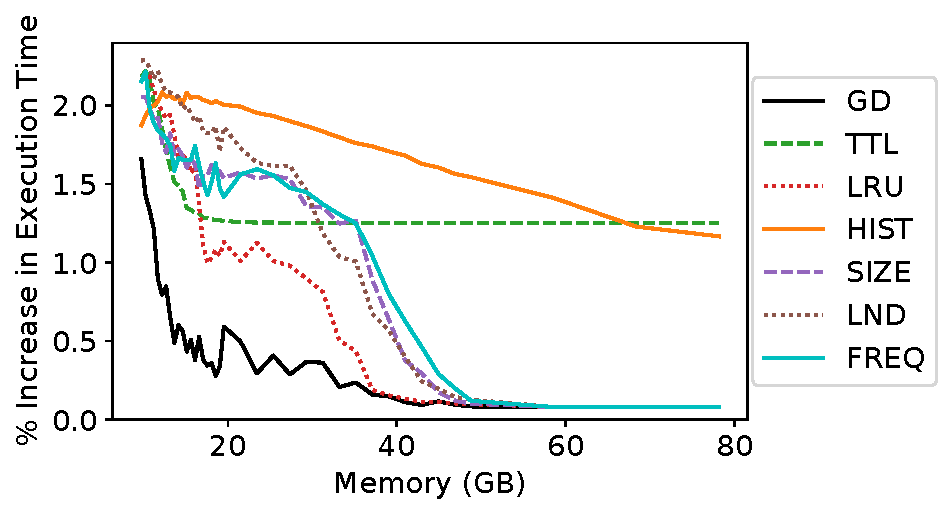
\includegraphics[width=0.37\textwidth]{faascache/faas-keepalive-20/graphs/rep-funcs-392/exec_inc_mem-392-legend.pdf}}
  \hfill 
    \subfloat[Rare functions.     \label{fig:rare-trace-exec}]
{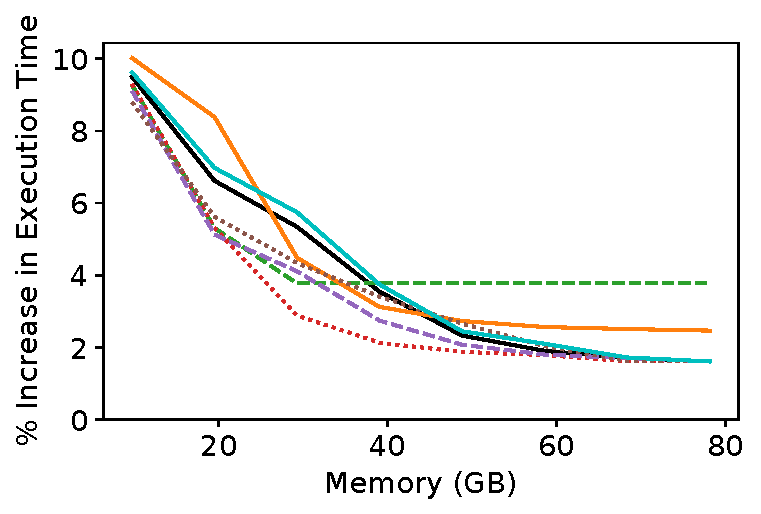
\includegraphics[width=0.3\textwidth]{faascache/faas-keepalive-20/graphs/rare-funcs-1000/exec_inc_mem-1000.pdf}}
\hfill 
  \subfloat[Random sampling.      \label{fig:random-trace-exec}] {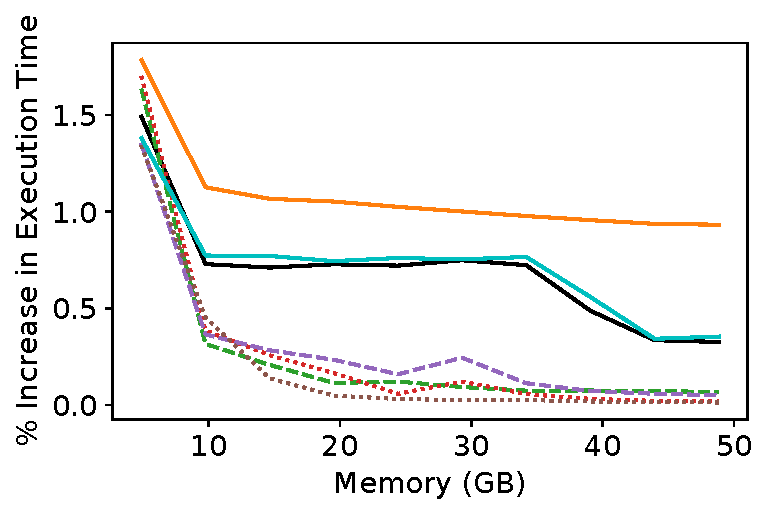
\includegraphics[width=0.3\textwidth]{faascache/faas-keepalive-20/graphs/random-funcs-200/exec_inc_mem-200.pdf}}
\caption{Increase in execution time due to cold starts for different workloads derived from the Azure function trace.}
\label{fig:exec-overheads-all}
\end{figure*}


\begin{figure*}[t]
  \centering
%  \vspace*{\myfigspace}
%  \begin{minipage}[c]{0.7\linewidth}
  \subfloat[Representative functions.\label{fig:rep-trace-cold}] {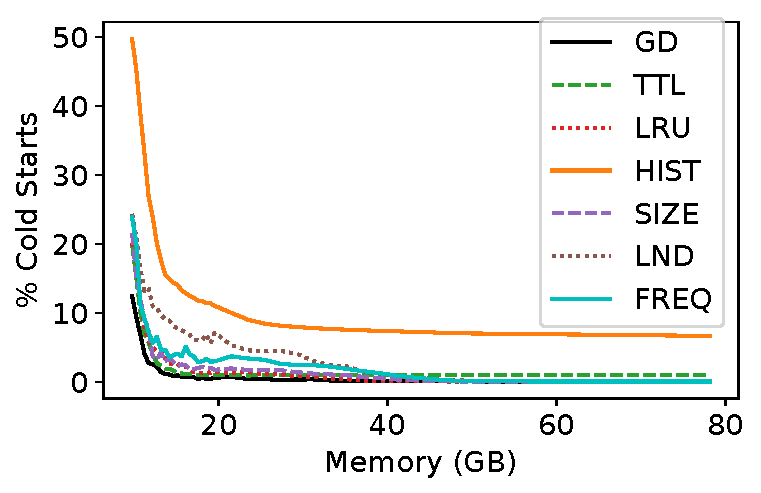
\includegraphics[width=0.33\textwidth]{faascache/faas-keepalive-20/graphs/rep-funcs-392/cold_drop_mem-392-legend.pdf}}
  \hfill
    \subfloat[Rare functions. \label{fig:rare-trace-cold}] {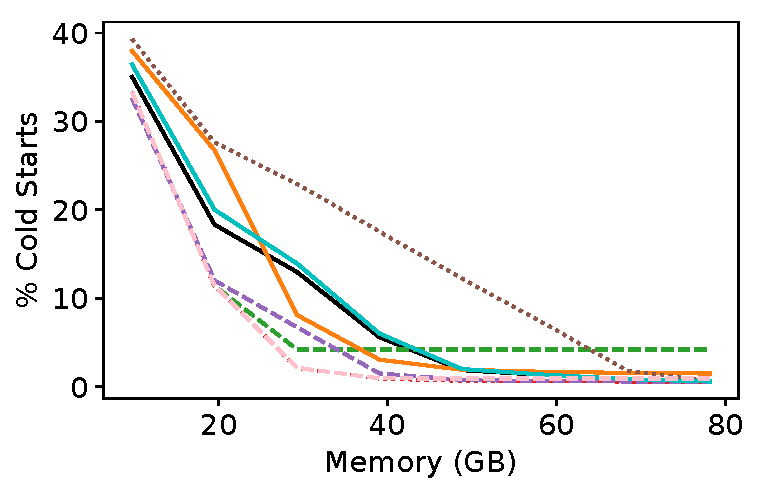
\includegraphics[width=0.33\textwidth]{faascache/faas-keepalive-20/graphs/rare-funcs-1000/cold_drop_mem-1000.pdf}}
  \hfill
  \subfloat[Random sampling. \label{fig:random-trace-cold}]
  {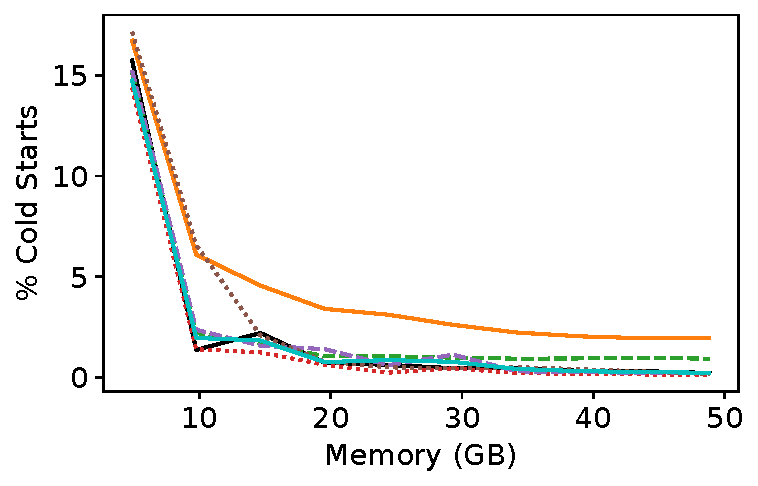
\includegraphics[width=0.33\textwidth]{faascache/faas-keepalive-20/graphs/random-funcs-200/cold_drop_mem-200.pdf}}
    \caption{Fraction of cold starts is lower with caching-based keep-alive. } % for different samples of the Azure function trace.}
      \label{fig:cold starts-all}
%    \end{minipage}
%    \hfill
%    \begin{minipage}[c]{0.29\linewidth}
 %      \begin{figure}
 %     \end{figure}
%    \end{minipage}
\end{figure*}


%%%%%%%%%%%%%%%%%%%%%%%%%%%%%%%%%%%%%%%%%%%%%%%%%%%%%%%%%%%%
\noindent \textbf{Setup, Workloads, and Metrics.}
%
For evaluating different keep-alive performance with different workload types, we use different trace samples from the Azure Function trace~\cite{shahrad_serverless_2020}, which contains execution times, memory sizes, and invocation-timestamps for more than 50,000 unique functions. 
Since our goal is to examine performance at a \emph{server} level, we use smaller samples of this trace for realistic server sizes, and replay them in our discrete-event keep-alive simulator. 
This also allows us to examine the behavior with different \emph{types} of workloads, which is important because our keep-alive policies are designed to be general and workload-agnostic.
We use the following three trace samples (more details in the Table~\ref{tab:trace-deets}): \\
\noindent \textbf{RARE:} A random sample of 1000 of the rarest, most infrequently invoked functions. These functions will usually result in cold starts under a classic 10 minute TTL.  \\
% mention 75% percentile detail?
\noindent \textbf{REPRESENTATIVE:} A sample of 400 functions, sampled from each quartile of the dataset based on frequency---yielding a more representative sample with higher function diversity. \\
\noindent \textbf{RANDOM:} A random sample of 200 functions.

% The FaasCache system is evaluated in Section~\ref{subsec:ow-eval}.
Functions from the FunctionBench~\cite{kim_functionbench_2019} suite are used for generating a realistic workload. 
A single server with 250 GB RAM and 48-core Intel Xeon Platinum 2.10 GHz CPUs is used for running all functions. The server is running modified OpenWhisk (i.e., FaasCache), and Ubuntu 16.04.5. 

\begin{table}
  \centering
  \caption{Size and inter-arrival time (IAT) details for the Azure Function workloads used in our evaluation.}
  \begin{tabular}{lrrr}
    \hline 
    Trace & Num Invocations & Reqs per sec & Avg. IAT \\
    \hline
    Representative & 1,348,162 & 190 /s & 5.4 ms \\
    Rare & 202,121 & 30 /s & 36 ms \\
    Random & 4,291,250 & 600 /s & 1.8 ms \\
    \hline
  \end{tabular}
  \label{tab:trace-deets}
\end{table}



\paragraph{Adapting the Azure Functions Trace.}
The format of the original Azure Function trace~\cite{shahrad_serverless_2020} requires some additional pre-processing and extrapolation for generating a workload.  
The full dataset consists of 14 days of function invocations, and billions of individual invocations. We use the first day's data, and do not consider functions that are never reused (i.e., with less than two invocations). 

The original trace provides memory consumption at the \textit{application} level---with the application made up of multiple functions.
Therefore, we evenly split the memory allocation between all functions in an application.
The dataset provides invocations in minute-wide buckets.
When injecting/replaying the workload, if there is only one invocation in a minute-bucket, it is injected at the beginning of the minute. 
For multiple invocations, they are equally spaced throughout the minute. 

%
The cold start overhead of each function is estimated as {\texttt maximum - average} runtime, and the execution times provided in the dataset are used for this computation. 
The dataset does not account for certain important sources of cold start overheads such as execution environment creation (e.g., Docker).
This unfortunately underestimates the cold start overheads.
However, because it applies uniformly to all functions, it preserves the relative performance of the different keep-alive policies, and does not affect the cache hit ratios. 
%

%These cold start overheads are generally constant, 

%This may not capture all the sources of cold start overhead such as the execution environment creation (e.g., Docker) and 

We are interested in two metrics: the cold start ratio; and the average increase in the execution time due to cold starts.
The increase in execution time is computed by averaging across all function invocations. 

%The latter captures the heterogeneity in function initialization overheads and invocation frequencies. 
%For estimating the time each function spends in explicit initialization, using the workload trace we subtract each functions' average runtime from its maximum runtime. 
%The dataset timings do not include provider overhead, so this initialization time is entirely due to application code.

%%
%Provider cold start overheads can be up to several seconds long, and take up the plurality of a function's execution time.
%Because the dataset does not include provider overhead, it is impossible to assign a realistic number to this cost.
%With these large penalties are not in our simulations, we therefore assume it as 0, but in reality the overhead is roughly constant.
%This causes the global increase in execution time to be smaller than it would be otherwise.
%Including a non-zero cold start cost would apply uniformly across all functions, and thus not change eviction priorities relative to one another.
%The cache hit ratio in Figure~\ref{fig:cold starts-all} would remain unchanged, and the Y-axis (the global increase in execution time) of Figure~\ref{fig:exec-overheads-all} would be scaled up relative to the chosen cold start overhead.
%%

% Using variable, real-world, times would require knowing or randomly assigning the runtime of functions, and would still require stochasticity as provider latency is not constant. 

% Not explaining this in the paper was our biggest “oops”: and there’s a few sources of confusion.
% Here is what we assumed: the dataset doesnt include container startup time, but the included function execution time captures both the function-initialization time (importing packages etc.), and the actual execution.
% So the assumption is that the Max execution time was due to this initialization overhead (which we include in the cold start overhead in our paper).
% The “time functions take to execute after they are ready to run” added to our confusion: we assumed this meant that it is the time when the control is transferred to the FaaS runtime inside the container: which would still incorporate all actual function initialization overheads.
% A contributing factor to making this assumptions was that most OpenWhisk applications do not have a strict explicit initialization, so it is in general not possible to know when a function is truly ready to execute non-idempotent code. 

% And so we end up with pretty small startup overheads, which can be seen from our Figure 5.
% Including container startup time and other overheads would make little difference to relative performance, since the extra overhead would apply to all functions.
% For instance, adding a constant startup penalty for all functions doesnt change their eviction priorities.
% The cache hit ratio (our Figure~\ref{fig:cold starts-all}) would remain unchanged, and the Y-axis of Figure~\ref{fig:exec-overheads-all} would be scaled up depending on the chosen cold start overheads. 

\begin{comment}
Our simulator evaluation uses real-world FaaS usage data from the recently released Azure Function trace~\cite{shahrad_serverless_2020}. 
The entire trace consists of tens of thousands of functions with billions of invocations, making it intractable to simulate the entire dataset.
Trace sampling methodology is important to capture the characteristics of the overall trace, and the scenarios where FaasCache is most effective.
Over half of all functions have an interval arrival time (IAT) over 30 minutes, where IAT is defined as execution time + idle time, guaranteeing them to always have cold starts when using a simple TTL eviction policy.
A tiny 1\% of functions account for nearly 90\% of all invocations, with an IAT of under a minute. 
% Therefore, smaller samples 
Given these extreme disparities, smaller samples must match behaviors of the larger dataset to show their effectiveness.
The full Azure trace can be suitably handled by a cluster of servers, in which case the system behavior is influenced by load-balancing and sharding policies, which our work is orthogonal to.
%Explain the rationale here. 
We generate three day-long traces using the Azure Functions dataset to showcase the effectiveness of FaasCache.
\prat{Insert reuse distance vs. time heatmaps for all these traces in the appendix along with table describing: number of fns, total invocations, avg. inter arrival time, etc.}
\end{comment}

%%%%%%%%%%%%%%%%%%%%%%%%%%%%%%%%%%%%%%%%%%%%%%%%%%%%%%%%%%%%
\subsection{Trace-Driven Keep-Alive Evaluation}

In this subsection, we use the Azure function traces to evaluate different keep-alive policies in our discrete-event simulator. 
% Primary Comparison? Competitors? 
We compare all caching-based variants against the default keep-alive policy in OpenWhisk (10 minute TTL).
% rev 1
When the server is full, this TTL policy evicts containers in an LRU order.
We also evaluate different Greedy-Dual variants: GD is our GDSF policy described in Section~\ref{subsec:gdsf}.
The others are the caching-based variants described in Section~\ref{subsec:variants}: LND is Landlord, and FREQ is LFU. 


%rev 1 
We also compare against the histogram-based keep-alive policy in~\cite{shahrad_serverless_2020}, which is the state of the art technique.
% Section 4.2 of serverless paper 
We have reproduced this policy (HIST) from the details in the paper, and have implemented it in a ``best-effort'' manner without any knowledge of the optimizations in the actual implementation.
This is effectively a ``TTL+Prefetching'' policy: it uses a histogram of \emph{inter-arrival times} to predict future function invocations and eagerly evict warm functions.
It uses timeseries forecasting to capture temporal locality, but does not consider the other function characteristics such as function size and initialization cost. 
The IAT, computed by taking a function's execution time plus the subsequent idle time, between each actual invocation is recorded in minute granularity buckets, tracking up to four hours between executions.
The policy uses ARIMA modeling for those invocations that fall outside this four hour window, we chose not to implement this specific feature due to its complexity, and the fact that it accounted for a minor fraction (\textasciitilde 0.56\%) of all invocations.
From these buckets, a function's coefficient of variation (CoV) is calculated using Welford's online algorithm~\cite{welford}. 
When the function's IAT is predictable (CoV $\leq 2$), the function's historical/customized preload and TTL time are used.
Otherwise, the function has a generic TTL of two hours. 
When an invocation is anticipated, it is brought into memory and kept there until its TTL expires.
A function is evicted when the policy predicts it will not have an invocation in the near future. 
%We chose not to implement the ARIMA modeling for IAT's exceeding four hours for simplicity and the fact it is only applicable to a tiny number of functions.
% \textbf{More details. Histogram size? When created? Online? }


%
The increase in execution time for different traces and for different cache sizes is shown in Figure~\ref{fig:exec-overheads-all}.
% How is this measured?
The increase in execution time is the cold start overheads averaged across all invocations of every function, and captures the user-visible response-time. 
%

For the representative trace (Figure~\ref{fig:rep-trace-exec}), Greedy-Dual reduces the cold start overhead by more than $3\times$ compared to TTL for a wide range of cache sizes (15--80 GB). 
Interestingly, it is able to achieve a low overhead of only 0.5\% at a much smaller cache size of 15GB, compared to other variants, which need 50 GB to achieve similar results---a reduction of cache size by more than $3\times$. 
%
For rare functions (Figure~\ref{fig:rare-trace-exec}), caching-based approaches such as LRU  reduce the cold start overhead by $2\times$ compared to TTL for cache sizes of 40--50 GB. 
This shows that for rare functions, recency is a more pertinent characteristic, and the complex four-way tradeoff used in Greedy-Dual is not necessarily ideal in all workload scenarios. 
For this workload, the HIST policy outperforms TTL, as reported in~\cite{shahrad_serverless_2020}. 
However, it results in 50\% higher cold start overhead compared to caching-based approaches.
Furthermore, because HIST uses only inter-arrival times, it is unable to perform well with heterogeneous representative workloads  (Figure~\ref{fig:rep-trace-exec}). 


Finally, the randomly sampled trace has a large number of infrequent functions because of the low probability of selecting the heavy-hitting functions.
In Figure~\ref{fig:random-trace-exec}, the recency component again dominates, and we see LRU outperforming other variants. 
The equivalence of LRU and TTL-based caching for rare objects has been noted~\cite{basu2017adaptive,jiang2018convergence}, which explains their similar behavior seen in Figure~\ref{fig:random-trace-exec}. 
%closeness of TTL and LRU performance for rare functions in our result. 


\noindent \emph{\textbf{Result:} For representative, diverse workloads, our GD policy can improve the performance and shrink cache sizes by up to $3\times$. For more homogeneous workloads, LRU can outperform current TTL-based approaches by $2\times$.}

%%%
% rev 1 
We can observe from Figure~\ref{fig:exec-overheads-all} that the increase in execution time is generally small ($<10\%$).
This is because of two main factors: the evaluation metric chosen, and the properties of the workload trace. 
The execution time is averaged across \emph{all} function invocations.
However, serverless workloads consist of a large number of very frequently invoked functions. 
The performance of these functions is generally not affected by keep-alive policies, since any policy is going to keep them in the cache because of their high frequency. 
Thus, the difference between non-work-conserving policies such as TTL and Greedy-Dual is masked because of the frequent and popular functions. 
For instance, the average inter-arrival time for all three workloads is less than 36ms, or about 27 function invocations per second. 
Thus, the server is overloaded, and TTL does well even though it is not work-conserving. 
As the IAT grows, the effectiveness of work-conserving caching-based approaches increases compared to TTL, as we shall see in the next subsection. 

%%%%
%While Figure~\ref{fig:exec-overheads-all} focuses on the average increase in execution latency, keep-alive can also reduce the tail latency of functions. Cold start 

%%%%

We see a similar relation and behavior in the miss-ratio curves shown in Figure~\ref{fig:cold starts-all}. 
Due to function heterogeneity, the cold start overheads are not strictly correlated with cache miss ratios, and thus the differences between policies is different compared to the previously described actual cold start overheads. 
% \prat{Write after colors are fixed.}
Classic miss-ratio curves do not consider the miss \emph{cost} (i.e., initialization cost), which is an important metric that is optimized by the Greedy-Dual approach.
Thus, in general, even in object caching contexts, miss-ratio curves deviate from the actual performance---a behavior that we also observe. 

%%%%%%%%%%%%%%%%%%%%%%%%%%%%%%%%%%%%%%%%%%%%%%%%%%%%%%%%%%%%
\subsection{OpenWhisk Evaluation}
\label{subsec:ow-eval}



\begin{figure}
  \centering
  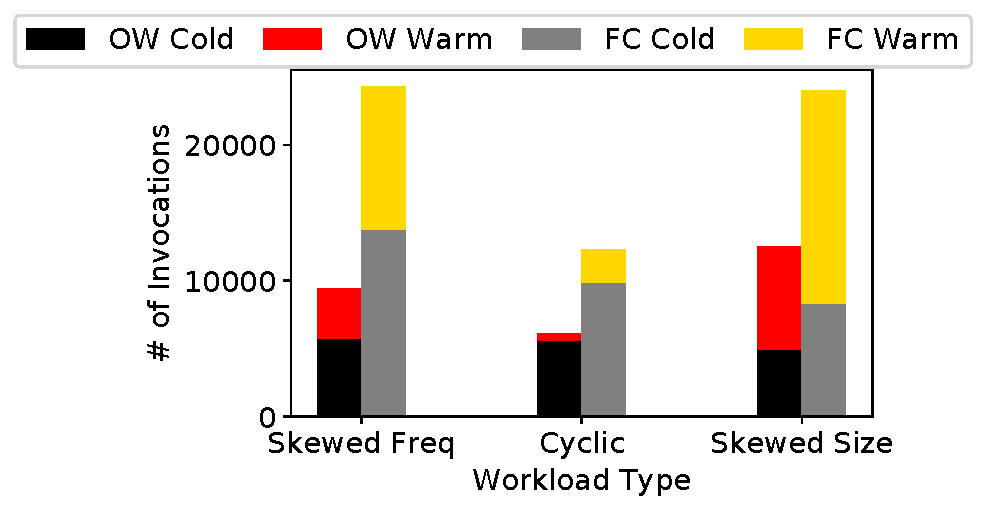
\includegraphics[width=0.6\textwidth]{faascache/faas-keepalive-20/graphs/litmus_tests/litmus_2_stacked.pdf}
  \caption{FaasCache runs 50 to 100\% more cold and warm functions, for skewed workload traces.}
  \label{fig:litmus_2}  
\end{figure}


In this subsection, we evaluate the performance of the FaasCache system on real functions. 
We focus on the performance of FaasCache's Greedy-Dual keep-alive implementation, and compare it to the vanilla OpenWhisk system which uses a 10 minute TTL.


% rev1 1
In contrast to the previous subsection in which we showed the average performance for different cache sizes, we will now also focus on the inverse problem: for a fixed server size, how much more load can be handled with FaasCache? 
By leveraging Greedy-Dual caching, FaasCache is able to reduce cold starts. 
This also reduces the number of \emph{dropped} requests. %

OpenWhisk buffers and eventually drops requests if it cannot fulfill them.
Because FaasCache more effectively selects evictions, its higher hit rate results in functions finishing faster, allowing more functions to be executed in the same time frame.  
%
\begin{table}
  \centering
  \caption{FaaS workloads are highly diverse in their resource requirements and running times. The initialization time can be significant and is the cause of the cold start overheads, and depends on the size of code and data dependencies.}
  \begin{tabular}{lrrr}
    \hline 
    Application & Mem size & Run time & Init. time \\
    \hline
    ML Inference (CNN) & 512 MB & 6.5 s & 4.5 s \\
    Video Encoding & 500 MB & 56 s & 3 s \\
    Matrix Multiply & 256 MB & 2.5 s & 2.2 s \\
    Disk-bench (\texttt{dd})  & 256 MB & 2.2 s & 1.8 s \\
    Image Manip & 300 MB & 9 s & 6 s \\
    Web-serving & 64 MB & 2.4 s & 2 s \\
    Floating Point & 128 MB & 2 s & 1.7 s \\
    \hline
  \end{tabular}
  % \vspace*{\myfigspace}
  \label{tab:fc:workloads}
  %\vspace*{\myfigspace}
\end{table}

To examine the effect of Greedy-Dual keep-alive on cold start and dropped requests, we use a workload trace comprising of four different functions: Disk-bench, ML inference, Web-serving, and Floating-point, described in Table~\ref{tab:fc:workloads}.

In Figure~\ref{fig:litmus_2}, we use different kinds of \emph{skewed} workloads: with a single function having a different frequency, a cyclic access pattern, and a skewed workload with 2 sizes. 
We see that FaasCache's keep-alive can increase the number of warm invocations by between 50 to 100\% compared to OpenWhisk's TTL.
The difference in the total number of requests served (warm+cold) is because OpenWhisk drops a significant number of requests due to its high cold start overhead and resultant system load. 
%
Thus with FaasCache, the total number of requests that are served also increases by $2\times$. 

%rev 1 above 
%Interestingly, OpenWhisk drops a significant number of requests, which is the cause of the different total served requests. 
%

% The impact on the different function performances can be seen in Figure~\ref{fig:faasbench}.
% For this figure, to generate the workload, the first three functions have an inter-arrival time of 1500 ms, and the fourth (floating-point) has a lower IAT of 400 ms. 

%a disk-based one, web-page serving, floating-point trigonomotry operations in numpy, and a convolutional neural network inference (TensorFlow with which model?). % A detailed description of these workloads is required.

% Explain what is the iat distribution and (other details? ).


% 32 GB wted_increase vanilla 11.964% cache 11.528%
% 48 GB wted_increase vanilla 6.184% cache 0.624%


\begin{figure}[t]
  \centering
\includegraphics[width=0.6\textwidth]{faascache/faas-keepalive-20/graphs/litmus_tests/faasbench_48_cold_hot-legend.pdf}
\caption{FaasCache increases warm-starts by more than $2\times$, which also reduces system load and dropped functions.}
\label{fig:faasbench}
\end{figure}


\begin{comment}
\begin{figure}[t]
  \centering
\subfloat[48 GB   \label{fig:faasbench-stacked-48}]
{ \includegraphics[width=0.3\textwidth]{../graphs/litmus_tests/faasbench_48_cold_hot-legend.pdf}}
\hfill 
  \subfloat[32 GB   \label{fig:faasbench-stacked-32}]
{  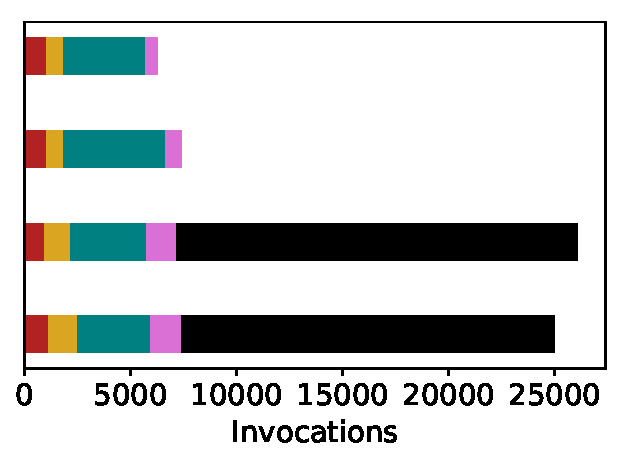
\includegraphics[width=0.17\textwidth]{../graphs/litmus_tests/faasbench_32_cold_hot.pdf}}
\caption{Impact of keep-alive on different function types.}
\label{fig:faasbench}
\end{figure}
\end{comment}

% Figure~\ref{fig:faasbench-stacked-32} shows the number of cold and dropped requests for the different functions, with a medium cache size of 32 GB.
% This setup is intended to evaluate our system in resource constrained environments.
% We see that dropped requests dominate, and FaasCache's more effective keep-alive serves 45\% of requests, while OpenWhisk only serving ~40\%.
% At the same time, warm starts improve 17\% using FaasCache.


Next, we use the skewed frequency workload and use functions from Table~\ref{tab:fc:workloads} to evaluate the impact on real applications. 
%The impact on the different function performances can be seen in Figure~\ref{fig:faasbench}.
To generate the workload, the CNN, DD, and Web-serving functions have an inter-arrival time of 1500 ms, and the Floating-point function has a lower IAT of 400 ms. 
%
Figure~\ref{fig:faasbench} shows the breakdown of different function invocations for this workload on a 48 GB server.
Interestingly, OpenWhisk drops a significant number (50\%) of requests due to the its high cold start overheads.
FaasCache increases the warm requests by more than $2\times$. 
Interestingly, the \emph{distribution} of warm starts is also different. 
FaasCache's Greedy-Dual policy prioritizes functions with higher initialization times, but penalizes those with large memory footprints. 
Because the floating-point function has a high initialization overhead (Table~\ref{tab:fc:workloads}), it sees a $3\times$ increase in hit-ratio compared to OpenWhisk.
\emph{In practical terms, the improvement in keep-alive results in a $6\times$ reduction in the application latency.
}
%The ML inference function has an 8\% lower warm hit rate than the other functions, as it gets de-prioritized because of it's high memory needs.


%When the cache size is increased to 48 GB (Figure~\ref{fig:faasbench-stacked-48}), FaasCache doesn't drop a single request, while OpenWhisk still can't serve 50\% of them.
%For the same workload, Figure~\ref{fig:faasbench-stacked-32} shows the distribution of cold and warm starts for a larger cache size of 32 GB.
%The number of warm starts increases by nearly 20\% compared to OpenWhisk.
% FaasCache's Greedy-Dual policy prioritizes functions with higher initialization times, the CNN function sees a 53\% higher warm starts, wheres Z function only sees X\% increase compared to OpenWhisk. 
% The floating point function has a very high initialization overhead (1.7 of the total 2 seconds), and thus sees its warm-start rate increase the most, by 40\%. 

\begin{comment}
At a smaller cache size of 32 GB shown in Figure~\ref{fig:faasbench-stacked-32}, the number of dropped requests dominate.
This setup is intended to evaluate our system in resource constrained environments.
FaasCache's more effective keep-alive serves 45\% of requests, while OpenWhisk drops nearly 60\%.
Warm-starts increase by 17\% with FaasCache. 
\end{comment}

\noindent \emph{\textbf{Result:} FaasCache can increase the number of warm-starts by $2\times$ to $3\times$ depending on the function initialization overheads and workload skew. This results in lower system load, which increases the number of requests FaasCache can serve by $2\times$.}

%\prat{CPU Graph not required, but just the average numbers will do.}

%%%%%%%%%%%%%%%%%%%%%%%%%%%%%%%%%%%%%%%%%%%%%%%%%%%%%%%%%%%%
\subsection{Effectiveness of Provisioning Policies}
All our previous results have been with a statically allocated server, and 
we now illustrate the effectiveness of our dynamic vertical scaling policy described in Section~\ref{subsec:dynamic}.
The goal is to dynamically adjust the cache size based on the workload. 
Our  policy seeks to keep the miss speed (cold starts per second) close to a pre-specified target. 
This is shown in Figure~\ref{fig:dynamic}---the target is 0.0015 misses per second. 
In this experiment, the cache resizing is done only when the miss speed error exceeds 30\%, and we can see that the cache size increases with the miss speed, and decreases with it. 
Without the dynamic scaling, a conservative provisioning policy would result in a constant, 10,000 MB size. 
In contrast, the average cache size with our proportional controller is less than 7,000 MB.
This 30\% reduction means that FaaS providers can reduce their provisioned resources without compromising on performance.
The freed-up resources can be used to accommodate additional cloud workloads (such as co-located VMs and containers). 
Our dynamic scaling is extremely conservative: increasing its agressiveness by reducing the error tolerance below 30\% will reduce  average server size,
%but cause a larger number of small memory-size  changes, which we wish to avoid.
but we seek to avoid the resultant small changes to memory-size to minimize fragmentation. 
%avoid why?? 

\begin{figure}[t]
  \centering 
  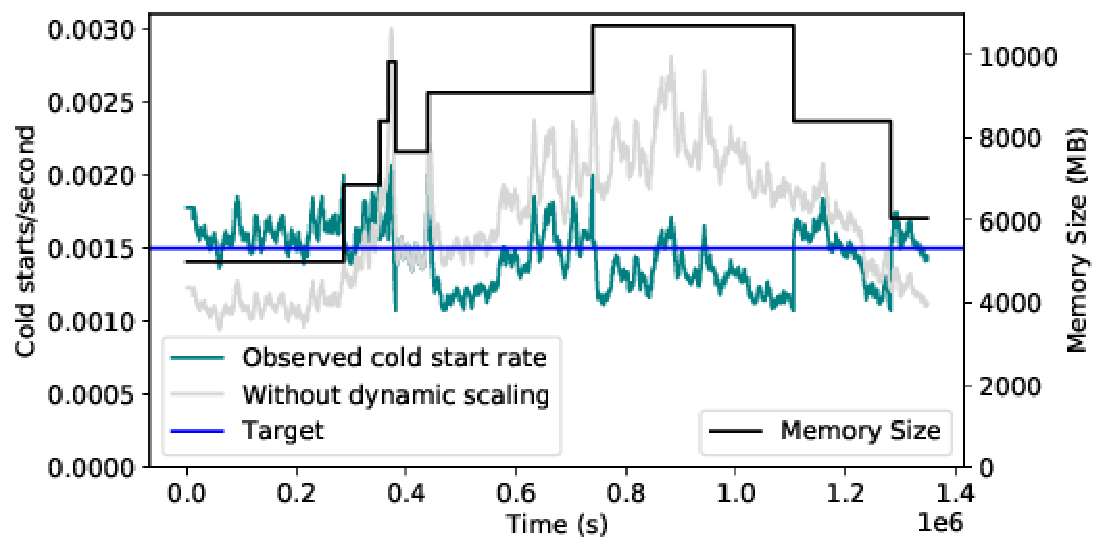
\includegraphics[width=0.6\textwidth]{faascache/faas-keepalive-20/graphs/dyn-scale-392-b.pdf}
  \caption{With dynamic cache size adjustment, the cold starts per second are kept close to the target (horizontal line), which reduces the average server size by 30\%. }
  \label{fig:dynamic}
\end{figure}

%%% Local Variables:
%%% mode: latex
%%% TeX-master: "paper"
%%% End:

% \vspace*{-8pt}
\section{Related Work}
\label{sec:related}

\noindent \textbf{Locality} is an important design and optimization principle in FaaS---and is a fundamental result of code and data initialization required for each function.
Keep-alive policies for warm-starts apply temporal locality~\cite{roy2022icebreaker, ebrahimi2024cold, vahidinia2022mitigating, shahrad2020serverless} and caching~\cite{faascache-asplos21, sundarrajan2017footprint} principles for the CPU memory pool; load balancing also benefits from stickiness~\cite{package-cristina-19, faaslb-hpdc22, abdi2023palette}.
Our work extends these principles to GPU functions via locality enhanced fair queuing and proactive memory management. 

% Bursty functions can cause load imbalance and queuing on systems, and intelligent queuing can avoid additional latency~\cite{yan2020hermes}.

\noindent \textbf{GPUs in serverless computing} is already a rich and fast-growing area of research. 
A big portion of prior work~\cite{naranjo2020accelerated, fingler2022dgsf, kim_gpu_2018} focuses on disaggregated accelerators, with GPUs accessed over the network using techniques such as rCUDA~\cite{duato2010rcuda}.
In contrast, we look at local GPUs without remote execution. 
Using FaaS-inspired abstractions to provide GPU acceleration as a service is also common: applications are broken down into kernels which can be run ``anywhere''.
Kernel-as-a-Service~\cite{pemberton2022kernel} and Molecule~\cite{du2022serverless} are two examples of this approach, where the main challenges are designing and providing efficient and usable API-remoting mechanisms. 
\cite{juan_reducing_2023} also uses remote memory pooling to address the exacerbated cold-start problems for GPUs, and also proposes parallel data-dependency and compute context prefetching through code-level optimizations. 
Paella~\cite{ng2023paella} similarly breaks apart model inference tasks into CUDA kernel launches to minimize scheduling ``bubbles''.
These and other recent~\cite{sage_zhao_towards_2024} specialized code-modifying techniques are orthogonal to our work, since we require general black-box functions.

% MIG Over-allocation causes fragmentation, and the opposite approach will reduce performance or prevent function execution due to insufficient resources.
% Assigned partitions can lead to underutilization due to fragmentation from poor placement and function idle periods. Idle functions cause immediate underutilization, which could be alleviated via temporal sharing complicating fixed hardware partition management even further.

The popularity of \textbf{ML inference} has resulted in a large number of specialized solutions to efficient GPU scheduling, which have similar challenges, but a different optimization spaces: inference resource requirements are much more deterministic~\cite{gujarati2020serving} and thus amenable to data-driven optimization~\cite{ali2022optimizing}, and the lack of isolation among requests provides many locality-enhancing and batching opportunities~\cite{yang2022infless, satzke2020efficient}. 
For instance, both FaST-GShare~\cite{gu2023fast} and TGS~\cite{tgs_wu2023transparent} leverage profiles of ML workloads to monitor GPU utilization and use 2d bin-packing (with time and memory dimensions) to schedule inference workloads.

%Both of these automatically move memory off of the device when kernels are done, and don't have to worry about applications holding onto device memory when idle.

%  profiles ML workloads to monitor how much of the GPU it utilizes, then uses this information to schedule inference tasks on GPUs to maximize utilization.
% ML inference tasks have fixed sized memory and kernel usages (known tensor sizes, etc.) and this is an effective approach.
% Other applications can have arbitrary and changing requirements, especially when one considers that function arguments are the main determiner of resource usage, so this idea breaks down when shifting to black-box applications.

Finally, \textbf{scheduling} is crucial for FaaS performance, with key tradeoffs in late vs. early binding~\cite{kaffes2021practical, kaffes_hermod_2022}.
Efficiency and fairness tradeoffs in GPU scheduling have been recently resolved~\cite{mo_optimal_2024}, but only in the offline context with a limited number of batch jobs with known utilities. 

%%% Local Variables:
%%% mode: latex
%%% TeX-master: "paper"
%%% End:

% \vspace*{-8pt}
\section{Conclusion}
%\vspace*{\subsecspace}

The main insight in this paper is the isomorphism between function keep-alive and object caching.
Using it, sophisticated caching policies can be applied to FaaS.
Our Greedy-Dual based keep-alive policy can reduce cold-start overheads by up to $4\times$ compared to simple policies.
The caching analogy can also be used to enhance resource provisioning. 


%\clearpage 
\balance

{
\bibliographystyle{acm}
\interlinepenalty=10000 %%%%For fixing url-related errors only 
\bibliography{faas,faas-asplos, lb}
%\bibliography{bagsjobs}
}

%\paragraph{OpenWhisk Evaluation Function Details.}


% The impact on the different function performances can be seen in Figure~\ref{fig:faasbench}.
% For this figure, to generate the workload, the first three functions have an inter-arrival time of 1500 ms, and the fourth (floating-point) has a lower IAT of 400 ms. 


We use the following functions from FunctionBench FaaS benchmark to run on OpenWhisk. 

\begin{enumerate}
  \item ML Inference: Image inference using the SqueezeNet CNN architecture, implemented in Tensorflow.
  \item Video Encoding: Download 11 MB mp4 file and convert it to a grayscale avi equivalent, using Python's cv2. 
  \item Matrix Multiplication: Using Numpy and \texttt{linalg.solve} of a randomly generated 20x20 matrix.
  \item Disk-bench: Read and write 1000 times from disk in 128k blocks using the \textbf{dd} command
  \item Web-serving: Generating and returning HTML for a small web page using Python's Chameleon. 
  \item Floating Point: A series of floating point trigonomotric computations using the standard Python math library.
\end{enumerate}



\paragraph{Azure Functions Dataset.}

We use the Azure function dataset to validate our keep-alive policies.
The full dataset consists of 14 days of function invocations, and billions of individual invocations. 
We use the first day's data, and do not consider functions with less than two invocations. 

Because memory is tracked at the \textit{application} level, and applications are made up of multiple functions, we evenly split the memory allocation between all functions in an application.


The dataset provides invocations in minute-wide buckets.
So when forming the traces, if there is only one invocation it is injected at the beginning of the minute.
For multiple invocations, they are equally spaced throughout the minute.

%Dataset location: https://github.com/Azure/AzurePublicDataset/blob/master/AzureFunctionsDataset2019.md

We use multiple different samples of this trace to validate our approach with different kinds of traces, and to make the analysis more tractable. We note that the full function trace is suitable for a large cluster of servers, whereas our focus is on a \emph{single} server.
The details of our trace samples are provided in Table~\ref{tab:trace-deets}. 
Figure~\ref{fig:whole-trace} shows the invocations/second of the full function trace (without sampling), and Figures~\ref{fig:392-trace}, \ref{fig:1000-trace}, and \ref{fig:200-trace} show the timeseries of our three workload traces. 
We can see that the representative trace (Figure~\ref{fig:392-trace}) captures the diurnal effects seen in the full trace (Figure~\ref{fig:whole-trace}).



\begin{table}
  \begin{tabular}{lrrr}
    \hline 
    Trace & Num Invocations & Reqs per sec & Avg. IAT \\
    \hline
    Representative & 1,348,162 & 190 /s & 5.4 ms \\
    Rare & 202,121 & 30 /s & 36 ms \\
    Random & 4,291,250 & 600 /s & 1.8 ms \\
    \hline
  \end{tabular}
  \caption{Size and IAT details for the three traces used in our evaluation.}
  \label{tab:trace-deets}
\end{table}


\begin{comment}

\begin{figure}[t]
  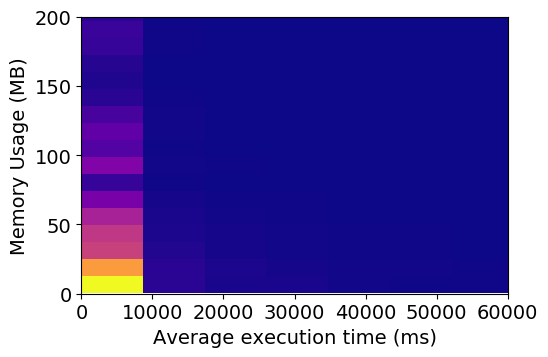
\includegraphics[width=0.3\textwidth]{../graphs/azure_analysis/mem-dur-corr.png}}
  \caption{Lack of correlation between a function's memory and average runtime duration}
  \label{fig:azure-mem-dur-corr}
\end{figure}

\begin{figure}[t]
  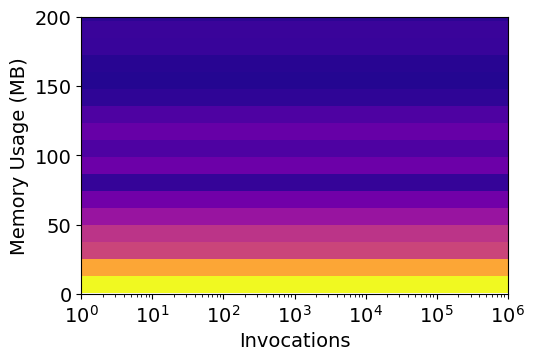
\includegraphics[width=0.3\textwidth]{../graphs/azure_analysis/mem-conv-corr.png}
  \caption{Lack of correlation between a function's memory and number of  times it is invoked}
  \label{fig:mem-invok-corr}
\end{figure}

\begin{figure}
    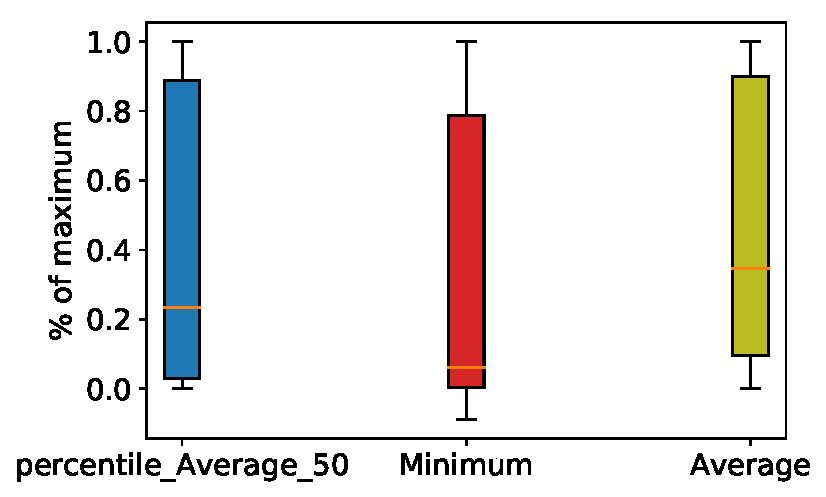
\includegraphics[width=0.3\textwidth]{../graphs/azure_analysis/cold_vs_warm.pdf}
    \caption{Relation between a functions maximum runtime and it's minimum, average, and 50th percentile average.}
    \label{fig:warm-cold-box}
\end{figure}

\end{comment}

\begin{figure}
 \centering 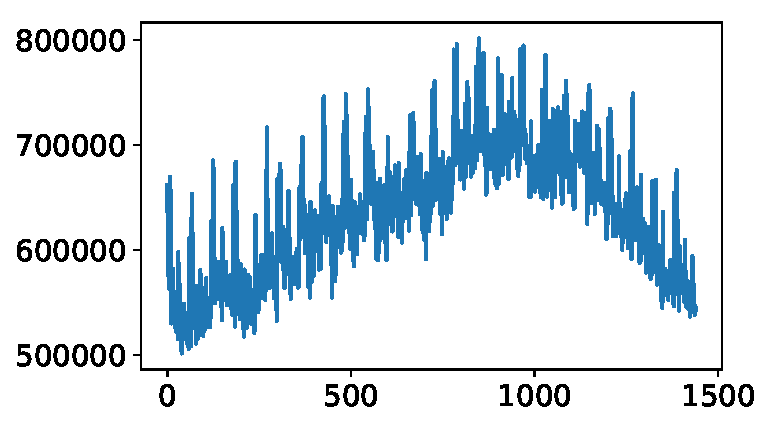
\includegraphics[width=0.3\textwidth]{../graphs/azure_analysis/whole_trace.pdf}
  \caption{Full Azure trace (Day 1) invocation timeseries.}
  \label{fig:whole-trace}
\end{figure}


\begin{figure}
 \centering   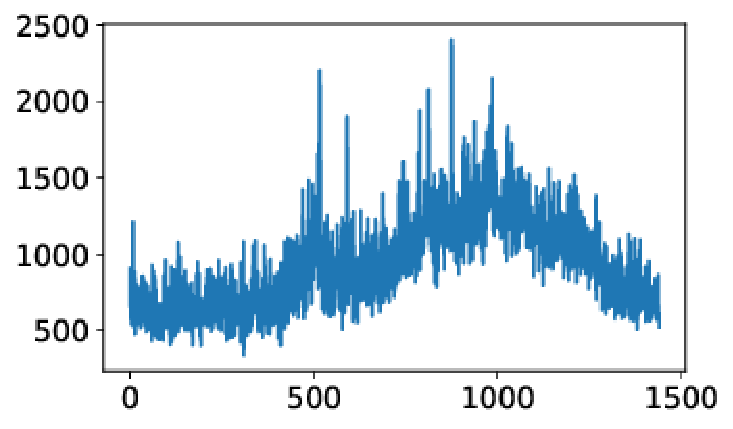
\includegraphics[width=0.3\textwidth]{../graphs/rep-funcs-392/392-b-trace.pdf}
  \caption{Representative trace invocation timeseries.}
  \label{fig:392-trace}
\end{figure}

\begin{figure}
  \centering  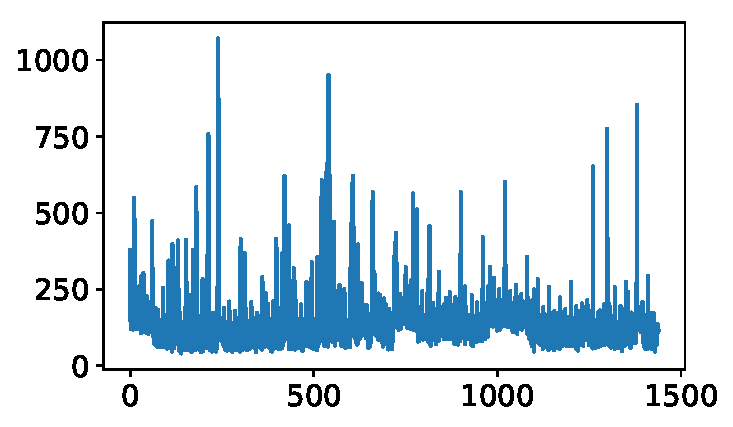
\includegraphics[width=0.3\textwidth]{../graphs/rare-funcs-1000/1000-b.pdf}
  \caption{Rare function trace invocation timeseries.}
  \label{fig:1000-trace}
\end{figure}


\begin{figure}
  \centering  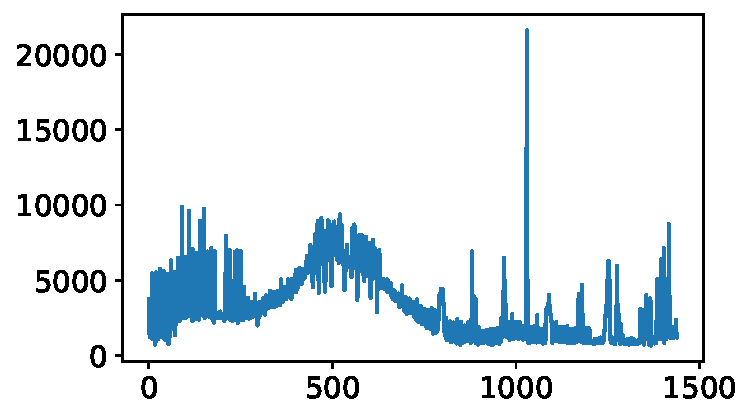
\includegraphics[width=0.3\textwidth]{../graphs/random-funcs-200/200-c.pdf}
  \caption{Randomly sampled trace invocation timeseries.}
  \label{fig:200-trace}
\end{figure}

%\end{comment}

%%% Local Variables:
%%% mode: latex
%%% TeX-master: "appendix-submit"
%%% End:


\end{document}


%%% Local Variables:
%%% mode: latex
%%% TeX-master: t
%%% End:

